\section{Statistical Analysis}\label{sec-fitFramework}
After collecting the data and various simulated samples, including detector effects, reconstructing the physics objects, and applying the complex selection and categorisation of events, the final step in the analysis is to measure the different \textit{Parameters of interest} (\gls{poi}) with the modelling strategy defined in the previous section. The combined analysis targets several deliverables to be measured, namely:
\begin{itemize}[leftmargin=*]
\item \textit{\vhb}: 
    \begin{itemize}
        \item Inclusive signal strength $\mu_{VH_{bb}}$ and significance: 1 \gls{poi}.
        \item Signal strengths for $WH(\rightarrow b\bar{b})$ and $ZH(\rightarrow b\bar{b})$: 2 \gls{poi}s.
        \item Fiducial \gls{stxs} measurements in the reduced stage 1.2, described in Section \ref{sec-modSignal} and Figure \ref{fig:model-stxsscheme}: 15 \gls{poi}s (8 for $ZH$, 7 for $WH$).
        \item Constraints on Yukawa Higgs-bottom coupling modifier $\kappa_b$. % TODO define this
    \end{itemize}
\item \textit{\vhc}:
    \begin{itemize}
        \item The signal strength $\mu_{VH_{cc}}$ and upper limits at the 95\% \gls{cl} : 1 \gls{poi}.
        \item Constraints on Yukawa Higgs-charm coupling modifier $\kappa_c$. % TODO define this
    \end{itemize}
\item \textit{Combined \vhbc}: 
    \begin{itemize}
        \item Effective field theory interpretation.
        \item Limits on the ratio of Yukawa coupling modifiers $\kappa_c / \kappa_c$. % TODO define this
    \end{itemize}
\end{itemize}

The \textit{signal strength or enhancement factor} $\mu$ is the ratio of the measurement signal yield to the expected yield in the \gls{sm}, from the process $\sigma_{VH} \times$ branching ratio of the decay targeted.

\subsection{Likelihoof Function Definition}\label{subsec-likelidef}
All parameters of interest are estimated by comparing theory-based expectations baked into \gls{mc}-simulated samples to real collected data in a fit. This fit is performed by maximising the binned-likelihood function in all the analysis regions simultaneously, as a function of the signal strengths and statistical and systematic uncertainties. The full binned-likelihood function is composed of three terms, accounting, respectively, for the number of events per bin $\mathcal{L}_{\text{Events}}$, the impact of systematics $\mathcal{L}_{\text{Systematics}}$, and finally the impact of the limited statistics of the simulated sample $\mathcal{L}_{\text{MC-stats}}$. These are combined into the likelihood function of Equation \ref{eq-simp-like-func}: 
\begin{equation}\label{eq-simp-like-func}
    \mathcal{L} = \mathcal{L}_{\text{Events}} \times \mathcal{L}_{\text{Systematics}} \times \mathcal{L}_{\text{MC-stats}}.
\end{equation}

The first part $\mathcal{L}_{\text{Events}}$ is statistically modelled with Poisson distributed ($\mathcal{P}$) probabilities for every bin $i$ in the analysis, comparing the number of measured data events $N_i$ to the expectations of the signal $s_i$ and backgrounds $b_i$ in simulations. The $\mu$ signals strengths \gls{poi}s enter this term as parameter modifying the expected signal contributions: \[\mathcal{L}_{\text{Events}} = \prod_{i\in \textrm{bins}} \mathcal{P}(N_i \,|\, \mu s_i + b_i) = \prod_{i\in \textrm{bins}} \frac{\left(\mu s_i + b_i\right)^{N_i}}{N_i} \, e^{-\left(\mu s_i + b_i\right)}.\] For \vhb, the several \gls{poi}s in the \gls{stxs} measurement sets the signal strengths as a vector $\boldsymbol{\mu}$ with one entry per \gls{stxs} bin.\\

The systematics uncertainties are introduced in the fit by the $\mathcal{L}_{\text{Systematics}}$ term as \gls{np} $\boldsymbol{\theta}$, accounting for possible perturbations to the expected signal and background yields $\{s_i, b_i\} \rightarrow \{s_i(\boldsymbol{\theta}), b_i(\boldsymbol{\theta})\}$ in each bin. The \gls{np}s are statistically modelled as standard Gaussian $\mathcal{N}(0, 1)$ penalties of mean 0 and unit-variance: \[ \mathcal{L}_{\text{Systematics}}(\boldsymbol{\theta}) = \prod_{\theta \in \boldsymbol{\theta}} \frac{1}{\sqrt{2\pi}} e^{- \theta^2/2}.\] The nominal value is by convention set at $\theta_0 = 0$, with $\theta = \pm 1$ representing a $\pm1$ $\sigma$ variation. The effect of each \gls{np} is determined in auxiliary measurements, following the prescriptions introduced in the modelling Sections \ref{sec-unc} and \ref{sec-mod}. For example, if an \gls{np} tracking the normalisation of a background with a 10\% prior is moved upwards by 1 standard deviation in the fit, the yield of the background is increased by 10\%. After the fit, the central values of the \gls{np}s can be moved upwards or downwards, with a deviation from the initial central value called a \textit{pull} and defined as \[ \text{pull}_{\theta} = \frac{\hat{\theta} - \theta_0}{\sigma_{\theta_0}}, \] where the prefit value $\theta_0 = 0 $ and $\sigma_{\theta_0} = 1$ for all \gls{np}s. The \textit{constraint} indicates the change in certainty on the \gls{np} after the fit, estimated by the variance $\sigma_{\hat{\theta}}$ measured in the inverse Hesse matrix at the maximal likelihood point. For the normalisation of the major backgrounds, special unconstrained \gls{np}s are included with no likelihood penalty and said to be \textit{free-floating} (\gls{fn}s). They are free to vary and determined from data in control regions with an enhanced purity of the processes they normalised. These special \gls{np}s and have prefit values $\theta_0$ set at 1. \\

The final part covers the uncertainties linked to the limited statistics of the \gls{mc}-samples, statistically modelling $\mathcal{L}_{\text{MC-stats}}$ with $\gamma$-parameters. One such $\gamma_i$ is introduced per bin, with the freedom to modify the expected background yield as $b_i(\boldsymbol{\theta}) \rightarrow \gamma_i b_i(\boldsymbol{\theta})$. The $\boldsymbol{\gamma}$ factors are Gaussian distributed with a likelihood function: \[\mathcal{L}_{\text{MC-stats}}(\boldsymbol{\gamma}) = \prod_{i\in \textrm{bins}} \mathcal{N} \left(\beta_i \,|\, \gamma_i\beta_i, \sqrt{\gamma_i\beta_i} \right),\] with $\beta_i = 1 / \sigma_{\text{rel}}^2$ introducing the relative statistical uncertainty ($\sigma_{\text{rel}}$) on the expected yield of the sum $b_i$ of backgrounds in bin $i$. \\

Bringing every component together, the full likelihood function of Equation \ref{eq-simp-like-func} is thus defined as
\begin{equation}
\mathcal{L}\left(\boldsymbol{\mu}, \boldsymbol{\theta}, \boldsymbol{\gamma}\right) = \prod_{i\in \textrm{bins}} \mathcal{P}(N_i \,|\, \boldsymbol{\mu} s_i(\boldsymbol{\theta}) + b_i(\boldsymbol{\theta}, \boldsymbol{\gamma})) \times  \prod_{\theta \in \boldsymbol{\theta}} \mathcal{N}(\theta \,|\, 0, 1) \times \prod_{i \in \textrm{bins}} \mathcal{N}(\beta_i \,|\, \gamma_i \beta_i, \sqrt{\gamma_i \beta_i}).
\end{equation}
The parameters $\{\boldsymbol{\mu}, \boldsymbol{\theta}, \boldsymbol{\gamma}\}$ jointly maximising the likelihood are written as $\{\hat{\boldsymbol{\mu}}, \hat{\boldsymbol{\theta}}, \hat{\boldsymbol{\gamma}}\}$ while those maximising the likelihood conditioned on a fixed value of $\boldsymbol{\mu}$ are written as $\{\hat{\hat{\boldsymbol{\theta}}}, \hat{\hat{\boldsymbol{\gamma}}}\}$. These two sets are used to define a profile likelihood ratio $\lambda(\boldsymbol{\mu})$ to test a certain hypothesis about the values of $\boldsymbol{\mu}$ with
\begin{equation}\label{eq-lik-ratio}
    \lambda(\boldsymbol{\mu}) = \frac{\mathcal{L}\left(\boldsymbol{\mu}, \hat{\hat{\boldsymbol{\theta}}}, \hat{\hat{\boldsymbol{\gamma}}} \right)}{\mathcal{L}\left(\hat{\boldsymbol{\mu}}, \hat{\boldsymbol{\theta}}, \hat{\boldsymbol{\gamma}} \right)}.
\end{equation}

The $\lambda$ ratio is bound to the range [0, 1], with higher values implying a good agreement between the data and the chosen $\boldsymbol{\mu}$ while lower values are signs of disagreements. This pattern permits the construction of a likelihood ratio test statistics $t_{\boldsymbol{\mu}}$, defined as \cite{asympForm}
\begin{equation}\label{eq-lik-ratio-test}
    t_{\boldsymbol{\mu}} =
      \begin{cases}
        -2 \ln \lambda(\boldsymbol{\mu}) & \hat{\boldsymbol{\mu}} \geq \boldsymbol{\mu} \\
        0 & \hat{\boldsymbol{\mu}} < \boldsymbol{\mu}
      \end{cases},
\end{equation}
since in this case, the signal can only have a positive contribution to the yield. This statistic is leveraged to perform two types of test: the no signal hypothesis $\boldsymbol{\mu} = \boldsymbol{0}$ and the nominal signal hypothesis $\boldsymbol{\mu} = \boldsymbol{1}$. In the no-signal hypothesis test, also called the null hypothesis, the $p$-value quantifies the compatibility of the observed data with a background-only hypothesis ($\mu = 0$). It is defined as:
\begin{equation}
    p_{\boldsymbol{\mu}}=\int_{t_{\boldsymbol{\mu},\mathrm{obs}}}^{\infty} f(t_{\boldsymbol{\mu}} \,| \, \boldsymbol{0}) dt_{\boldsymbol{\mu}},
\end{equation}
where $t_{\boldsymbol{\mu},\mathrm{obs}}$ is the observed test statistics (for the observed $\hat{\boldsymbol{\mu}}$) and $f(t_{\boldsymbol{\mu}} \,| \,0)$ is the test statiscs $t_{\boldsymbol{\mu}}$ probability density function assuming $\boldsymbol{\mu} = \boldsymbol{0}$. The $p$-value is the probability of finding data that is equally or more incompatible with the null hypothesis. Therefore, a low $p$-value gives confidence to reject the null hypothesis. In particle physics, the $p$-value is often translated into the significance $Z$, measuring the number of Gaussian standard deviations ($\sigma$) above the background as
\begin{equation}
    Z = \Phi^{-1}(1-p_{\boldsymbol{\mu}}),
\end{equation}
where $\Phi^{-1}$ is the inverse Gaussian cumulative distribution function. The standard for \textit{observation} of a process is arbitrarily set by the community at 5 $\sigma$ (correspond to a $p$-value $\approx 3 \times 10^{-7}$), with a 3 $\sigma$ signal strength significance ($p$-value $\approx 10^{-3}$) taken as \textit{evidence} of a process.  \\

To determine a 95\% upper limit \gls{cl} on a signal strength, a modified frequentist \gls{cl}$_s$ method is deployed \cite{asympForm, ALRead_2002}, based on the test statistics $\tilde{t}$ defined as:
\begin{equation}
    \tilde{t} = -2 \ln \frac{\mathcal{L}_{s+b}}{\mathcal{L}_{b}} = -2 \ln \frac{\mathcal{L}\left(\mu = 1, \hat{\hat{\boldsymbol{\theta}}}(\mu = 1), \hat{\hat{\boldsymbol{\gamma}}}(\mu = 1) \right)}{\mathcal{L}\left(\mu = 0, \hat{\hat{\boldsymbol{\theta}}}(\mu = 0), \hat{\hat{\boldsymbol{\gamma}}}(\mu = 0) \right)},
\end{equation}
where $\mathcal{L}_{s+b}$ is the nominal signal hypothesis ($\mu = 1$) and $\mathcal{L}_{b}$ the null hypothesis ($\mu = 0$), with the conditional likelihood optimisation of $\boldsymbol{\theta}$ and $\boldsymbol{\gamma}$ distinct between the two hypotheses for $\mu$. The upper 95\% \gls{cl}$_s$ limit on the signal strength $\mu$ is the $\mu$ value such that the $p$-value of the test statistics $\tilde{t}$ is equal to 0.05.\\

In addition to the fits performed between real and simulated datasets, so-called \textit{Asimov} fits are performed. These leverage the \textit{Asimov} datasets, corresponding to the sum of all simulated processes (signal + backgrounds). Two such sets are used: a \textit{prefit} Asimov dataset where the nuisance parameters are set to their initial values\footnote{0 for all \gls{np}s but the \gls{fn}s, which are set at 1.}, and a \textit{postfit} Asimov dataset where the \gls{np}s take their best-fit values from the fit to the real dataset. The postfit Asimov dataset can be used to define expected results, which quantify the sensitivity of the analysis to any similarly collected real data. Fits can be performed either conditionally or unconditionally, by setting the \gls{poi}s to their \gls{sm} expectations or letting them free-floating. 

\subsection[The \vhbc\ Fit]{The \boldvhbc\ fit}\label{subsec-subsecVHBCfit}
There are 15 \gls{poi}s for the \vhb\ side and 1 \gls{poi} for \vhc. The binning used and regions included as well as the variables defining the underlying distributions entering the fits are detailed in Sections \ref{sec-selectionandcat} and \ref{sec-vh-disc}. A dense summary of the full categorisation is presented in Figure \ref{fig:ana-strat-det}, underscoring the complexity of an analysis spanning 164 different regions, 84 of which are in \vhc\ (30 \gls{sr}s, 6 Top $e\mu$ \gls{cr}s, 10 $V+l$ \gls{cr}s, 48 CRHigh), 48 in the resolved \vhb\ (21 \gls{sr}s, 6 CRLow, 21 CRHigh), 12 $BT$-tagged Top \gls{cr}s shared in the resolved regime, and 10 in the boosted regime (6 \gls{sr}s, 4 boosted Top \gls{cr}s). Experimental and modelling uncertainties are introduced to account for any mis-modelling and avoid biasing the fit, as described in Sections \ref{sec-unc} and \ref{sec-mod}. The analysis described in this thesis is not yet concluded, with modifications to the modelling under active investigation at the time of writing. Consequently, the fit is still blinded, with the data in signal regions bins most sensitive to the signal hidden. For $m_{bb}$ or $m_{cc}$ distributions, the $H$-mass peak is blinded from 70 GeV to 140 GeV. For the \gls{mva} distributions, right-most (thus most signal-like) bins are iteratively blinded until at least 60\% of the signal yield in the region is contained in blinded bins. For conditional fits, these blinded bins are used but the data is still not displayed in the plots. This thesis does not describe any unconditional fit to data, with any unconditional fits included performed with the Asimov dataset instead of the real data. % As such, the results presented here correspond to the expected results from the postfit Asimov.  % Final sentence not clear: what am I showing?

\subsubsection{\boldvhc}
Concerning the \vhc\ signal strength measurement, the 95\% \gls{cl}$_s$ expected upper limits are shown for the different lepton channels and combined in Figure \ref{fig:fit_new_vhcclimitPostfit} for the postfit Asimov and Figure \ref{fig:fit_new_vhcclimitPrefit} for the prefit Asimov. %To compare, the published ATLAS \vhc\ result is shown in Figure \ref{fig:fit_old_vhcclimit} \cite{Collaboration:2721696}.

\begin{figure}[h!]
    \centering
    %\begin{subfigure}[b]{0.32\textwidth}
    %    \centering
    %    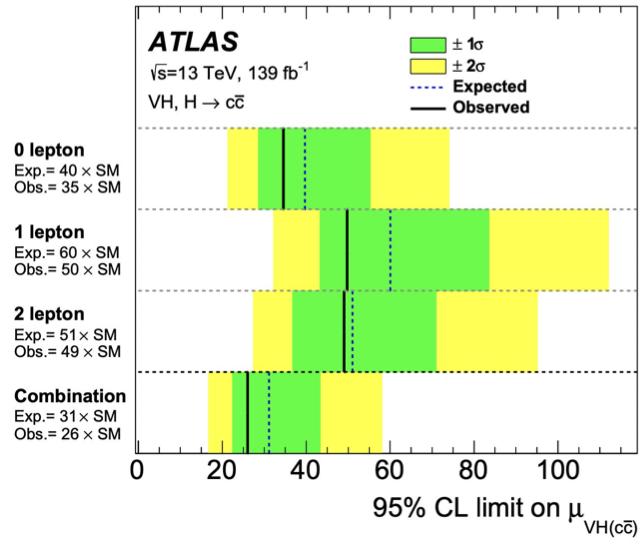
\includegraphics[width=\textwidth]{Images/VH/Fit/fromSlides/oldVHcc.%png}
    %    \caption{\vhc\ analysis \cite{Collaboration:2721696}.}
    %    \label{fig:fit_old_vhcclimit}
    %\end{subfigure}
    \begin{subfigure}[b]{0.48\textwidth}
        \centering
        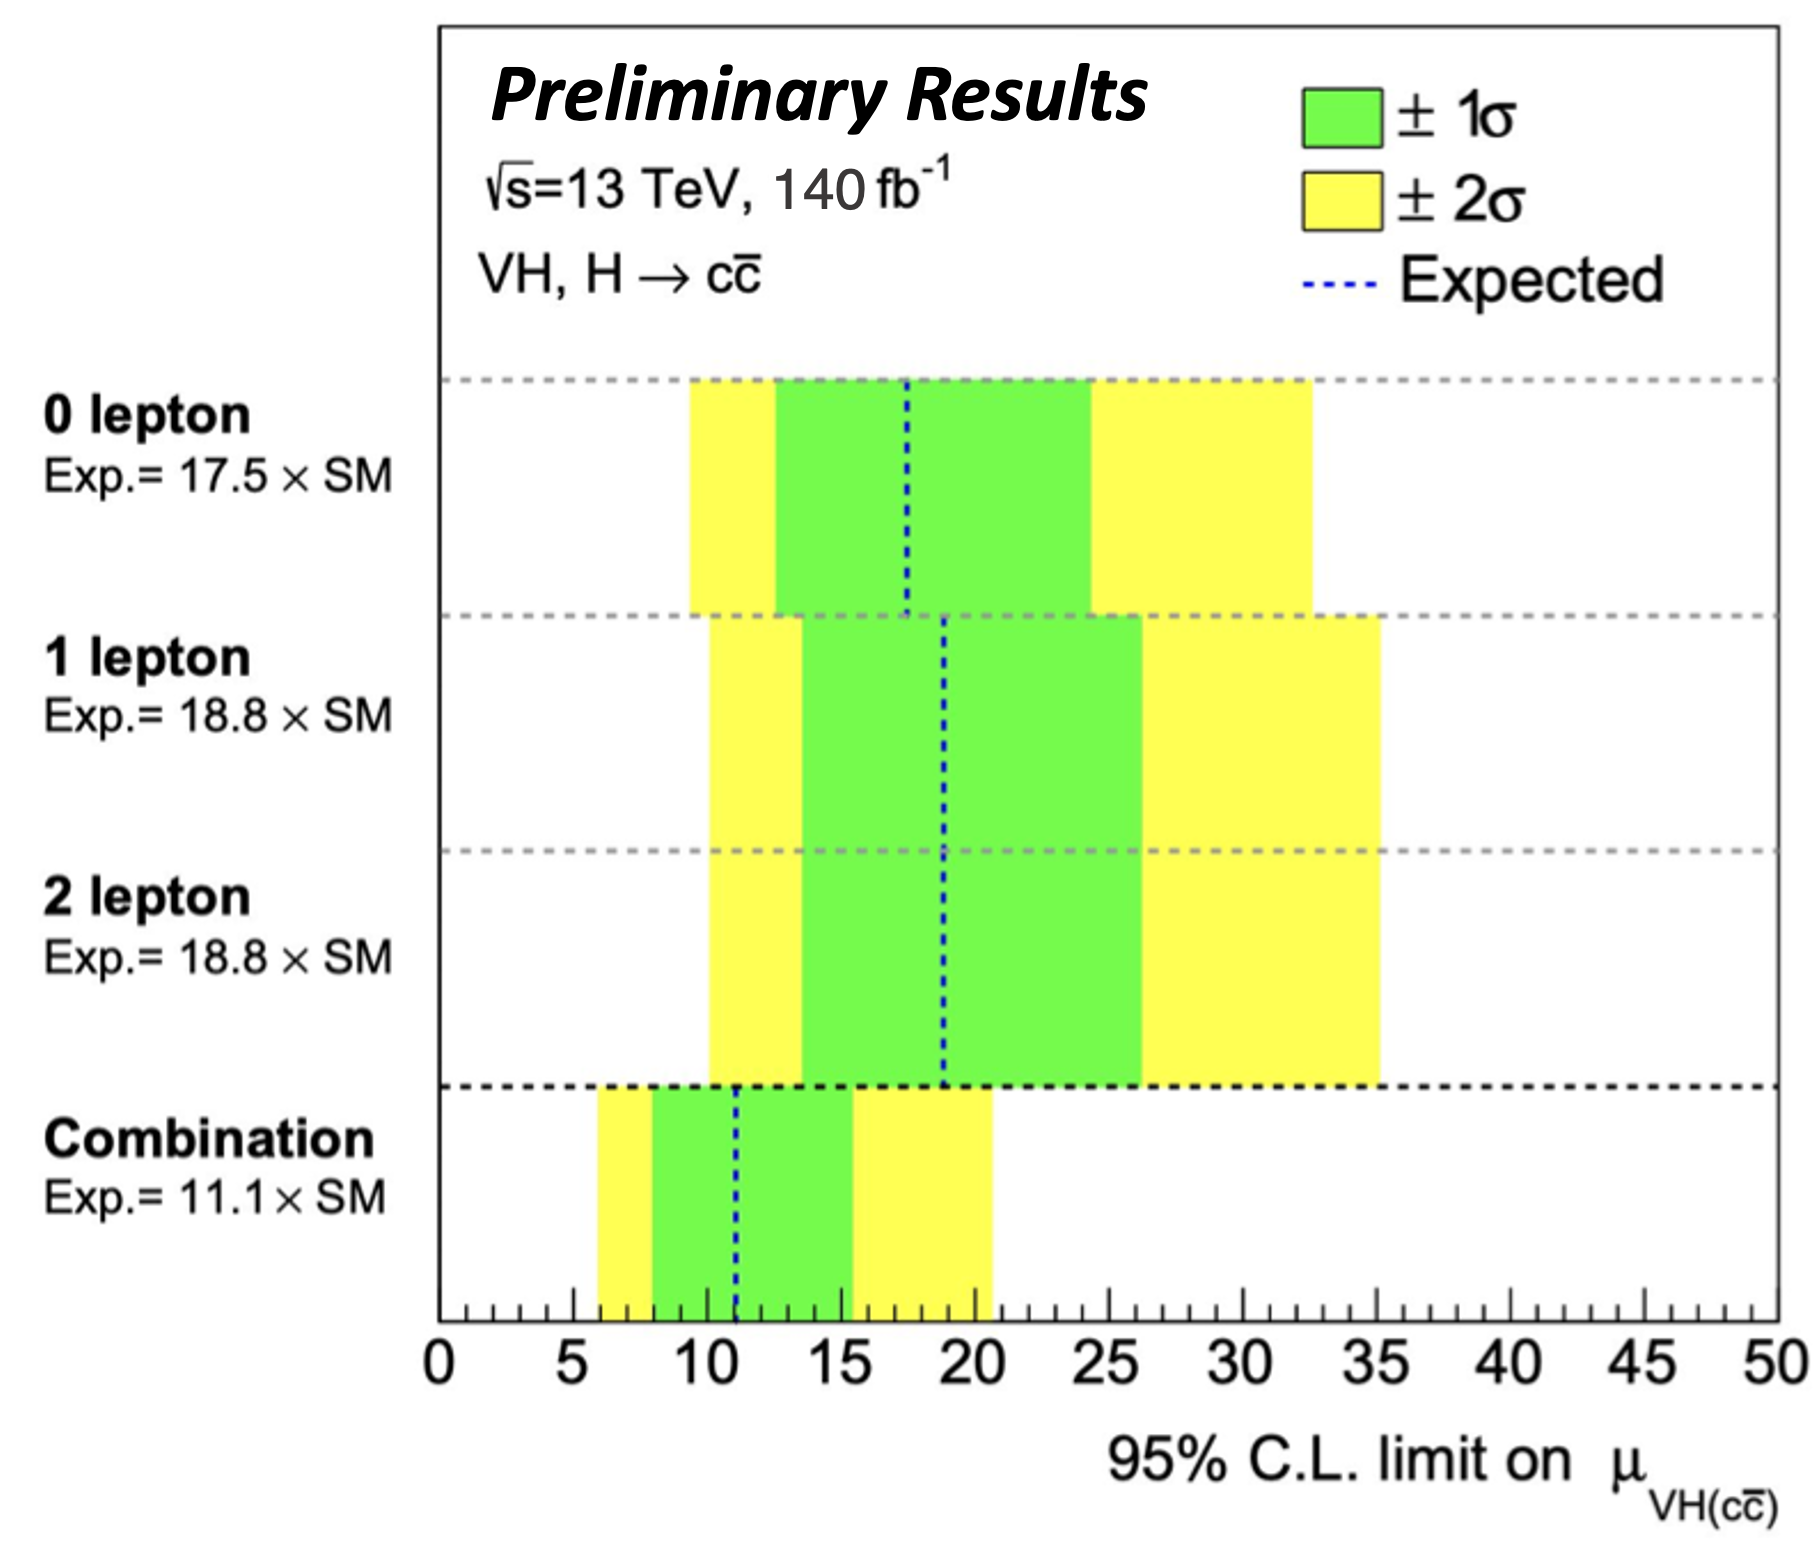
\includegraphics[width=\textwidth]{Images/VH/Fit/fromSlides/postfitVHcc.png}
        \caption{Combined postfit Asimov.}
        \label{fig:fit_new_vhcclimitPostfit}
    \end{subfigure}
    \begin{subfigure}[b]{0.48\textwidth}
      \centering
      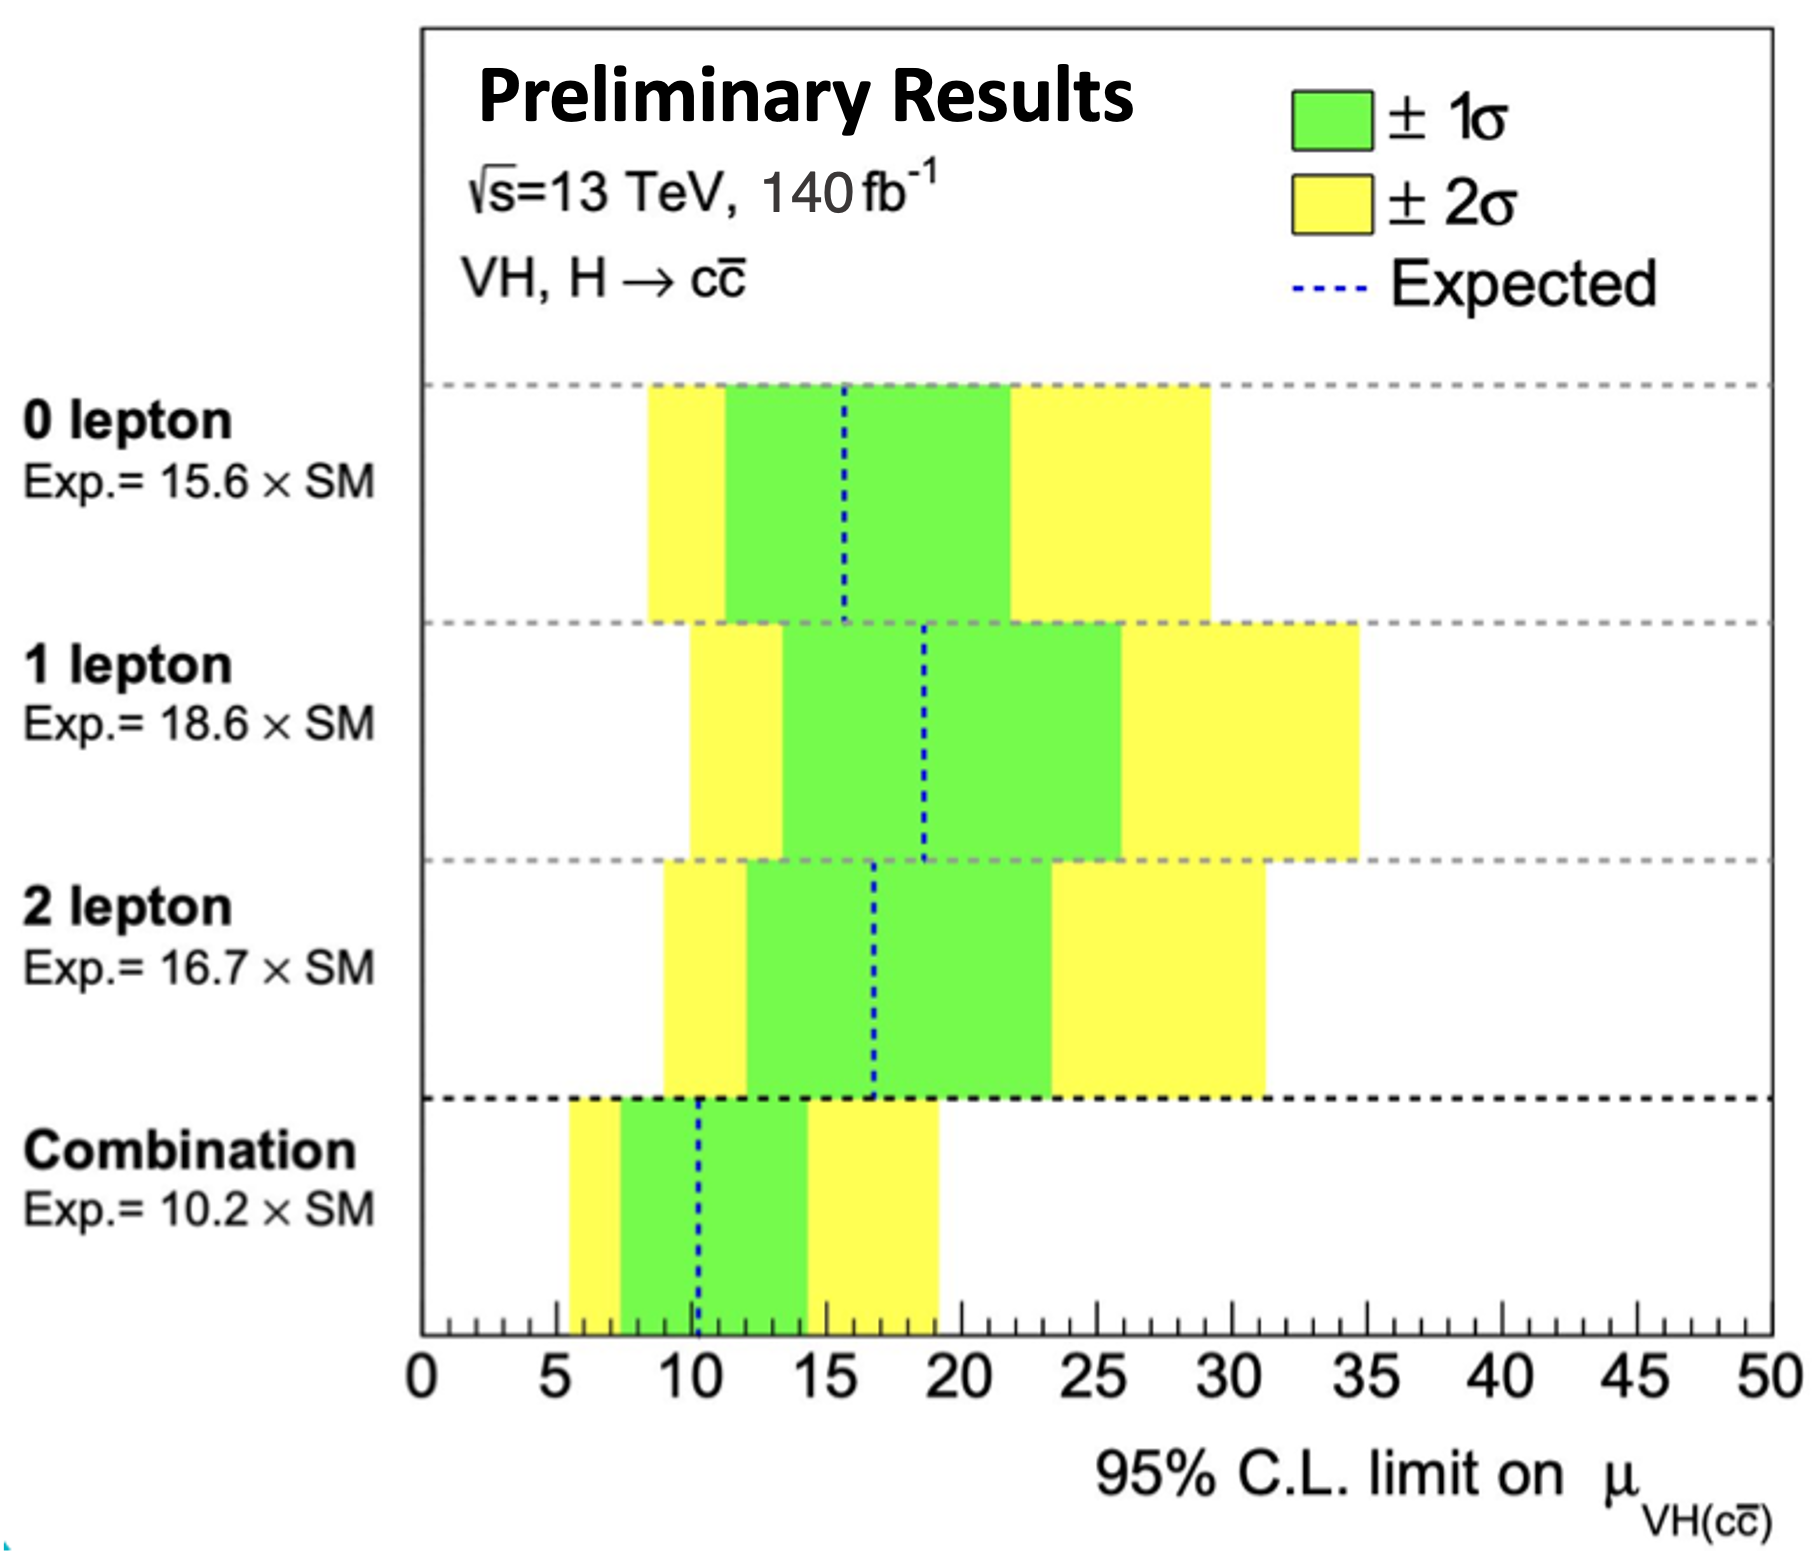
\includegraphics[width=\textwidth]{Images/VH/Fit/fromSlides/prefitVHcc.png}
      \caption{Combined prefit Asimov.}
      \label{fig:fit_new_vhcclimitPrefit}
  \end{subfigure}
    \caption{The 95\% CL$_s$ upper limit on the \vhc\ signal strength from the combined analysis posfit (left) and prefit (right).}
    \label{fig:fit_vhcc_limits}
\end{figure} 

Significant improvements are expected for all lepton channels. The combination of all lepton channels leads to a remarkable improvement on the 95\% \gls{cl}$_s$ upper limit on $\mu_{VHcc}$ from 31 $\times$ \gls{sm} in the latest published ATLAS \vhc\ analysis \cite{Collaboration:2721696} to 11.1 $\times$ \gls{sm} (10.2 $\times$ \gls{sm}) in the postfit (prefit) Asimov combined one, a factor 2.8 improvements in sensitivity. Gains are expected to be made in all lepton channels, which now have very similar sensitivity thanks to modifications to the analysis strategy. Compared to the published analysis, the 0-lepton channel upper limit is reduced from 40 $\times$ \gls{sm} $\rightarrow$ 17.5 $\times$ \gls{sm}, the lepton from 60 $\times$ \gls{sm} $\rightarrow$ 18.8 $\times$ \gls{sm}, and the 2-lepton from 51 $\times$ \gls{sm} $\rightarrow$ 18.8 $\times$ \gls{sm} \cite{Collaboration:2721696}. These correspond to relative sensitivity improvement factors of 2.3, 3.2, and 2.7. Most of the gains are made in the 1- and 2-lepton channels, although the 0-lepton channel remains the most sensitive one.

%\subsubsection{\vhb}
\subsubsection{\boldvhb}
On the \vhb\ side, combining the resolved and boosted regime, the postfit expected significance on the \vhb\ signal strength is 7.9 $\sigma$ over the background-only prediction, corresponding to a 23\% improvement over the published expected significance at 6.3 $\sigma$ \cite{ATLAS:2021wqh}. This is achieved thanks to a postfit expected significance of 4.7 $\sigma$ in the 0-lepton channel (15\% improvement to published result), 5.3 $\sigma$ in 1-lepton (30\% improvement), and 4.4 $\sigma$ in 2-lepton (3\% improvement). The most sensitive channel is distinctively the 1-lepton channel in this case. \\% check the 2L improvement, seems low

Separating the \vhb\ signal strength into two \gls{poi}s for $WH(H \rightarrow{b\bar{b}})$ and $ZH(H \rightarrow{b\bar{b}})$, the prefit expected significances are 5.5 $\sigma$ for $WH$ and 6.2 $\sigma$ for $ZH$. This marks the first time a $H \rightarrow b\bar{b}$ analysis is expected to reach observation-level in $WH$, thanks to the large improvement in the 1-lepton channel sensitivity. \\

Finally, adopting the fine splitting of the \gls{stxs} stage 1.2 with 15 bins defined by \ptv\ and additional jet multiplicity \nj, with 8 bins in $ZH$ and 7 bins in $WH$, the \vhb\ analysis reaches the per bin sensitivities listed in Table \ref{tab:exp-stxs-prefit}, with evidence-level only attained for the 150 GeV < \ptv\ < 250 GeV with no additional jet $ZH$ bin. The impact of systematics and statistical uncertainties on the signal strengths of the different bins is shown in Figure \ref{fig:fit-stxs-cons}.

\begin{table}[h!]
    \centering
    \renewcommand*{\arraystretch}{1.3}
    \begin{tabular}{c r | C{4cm} C{4cm}}
        \hline \hline
        $VH$ & \multicolumn{1}{c|}{Truth \ptv} & 0 additional \nj & $\geq$1 additional \nj \\
        \hline
        WH &  [75, 150[ GeV & \multicolumn{2}{c}{0.69 $\sigma$} \\
        WH & [150, 250[ GeV & 2.29 $\sigma$ & 0.55 $\sigma$ \\
        WH & [250, 400[ GeV & 2.78 $\sigma$ & 0.94 $\sigma$ \\
        WH & [400, 600[ GeV & \multicolumn{2}{c}{1.87 $\sigma$} \\
        WH & $\geq$ 600 GeV & \multicolumn{2}{c}{1.43 $\sigma$} \\ \hline

        ZH &  [75, 150[ GeV & 1.48 $\sigma$ & 0.90 $\sigma$\\
        ZH & [150, 250[ GeV & 3.37 $\sigma$ & 1.64 $\sigma$ \\
        ZH & [250, 400[ GeV & 2.85 $\sigma$ & 1.49 $\sigma$ \\
        ZH & [400, 600[ GeV & \multicolumn{2}{c}{1.91 $\sigma$} \\
        ZH & $\geq$ 600 GeV & \multicolumn{2}{c}{1.07 $\sigma$} \\ 
        \hline \hline
    \end{tabular}
    \caption{The expected prefit significance in the different STXS bins of the combined analysis.}
    \label{tab:exp-stxs-prefit}
\end{table}

\begin{figure}[h!]
    \centering
    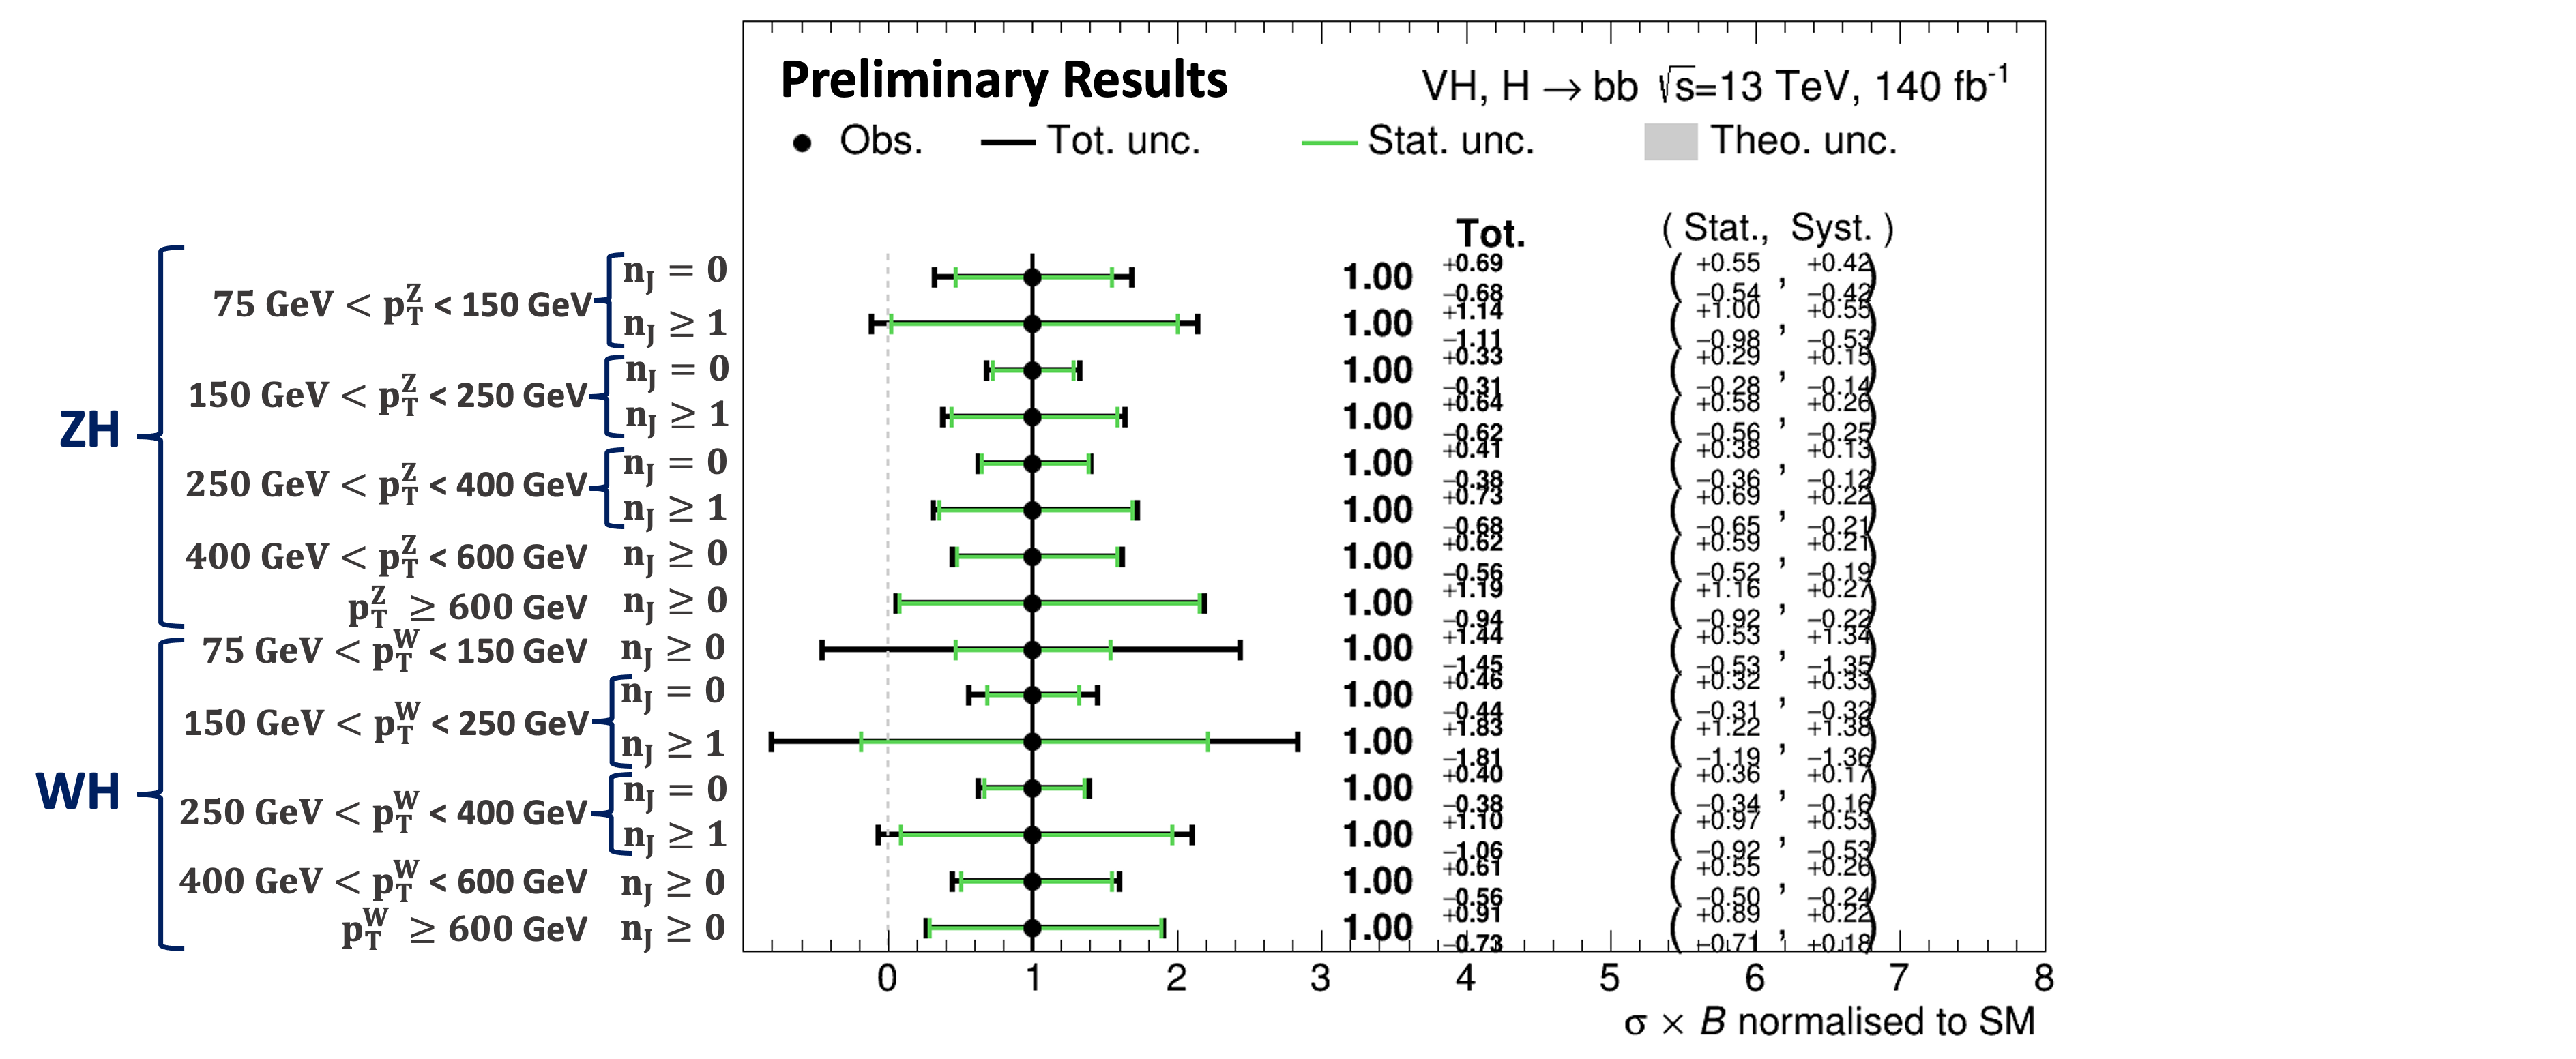
\includegraphics[width=\textwidth]{Images/VH/Fit/fromSlides/STXS_cons.png}
    \caption{The constraints on the prefit STXS signal strength.}
    \label{fig:fit-stxs-cons}
\end{figure} 

\subsubsection{The Diboson Cross-Check}\label{subsec-DibosonC}
The diboson cross-check analysis is performed with the $VZ (\rightarrow b\bar{b})$ and $VZ (\rightarrow c\bar{c})$ as signals in a similar fashion to the \vhbc\ fit, to validate the strategy adopted. For the $VZ (\rightarrow b\bar{b})$ part, the postfit expected significance reaches a large value of 15.1 $\sigma$ when combining lepton channels. The 0-lepton channel reaches 11.2 $\sigma$, 1-lepton 6.2 $\sigma$, and 2-lepton 9 $\sigma$. On the $VZ (\rightarrow c\bar{c})$ side, the combined analysis expects to reach observation level for the first time, with a combined postfit expected significance of 5.1 $\sigma$. This represents a significant improvement of a factor 2.3 from the 2.2 $\sigma$ published expected result \cite{Collaboration:2721696}. The combined analysis reaches a postfit expected significance of 3.9 $\sigma$ in 0-lepton, 2.6 $\sigma$ in 1-lepton, and 3.1 $\sigma$ in 2-lepton.

\subsubsection{Additional Fit Results}
In addition to the main results highlighted above, some further insights into the output of the fits are given before concluding this chapter. To verify the \gls{mc}-samples correctly reproduce the data after the fit, some posfit plots are presented in Figure \ref{fig:postfit_SR_CR} for selected signal regions and control regions, with all of them listed in Appendix \ref{appsec-vh-analRegPosfit}. Interestingly, good agreement between the data and posfit \gls{mc} samples is also observed for validation distributions not directly constrained in the fit. Figure \ref{fig:postfitval} displays posfit distributions for a $BL$-tagged region analoguous to the used $BT$-tagged Top CR, an $LL$-tagged region similar to a $c$-tagged signal region, and the \ptv\ spectrum of the whole 2L $BB$-tagged 2-jet signal region. The good agreement observed between data and \gls{mc}-samples in all regions is a sign of the correct constraining by the fit. \\

\begin{figure}[h!]
    \centering
    \begin{subfigure}[b]{0.32\textwidth}
        \centering
        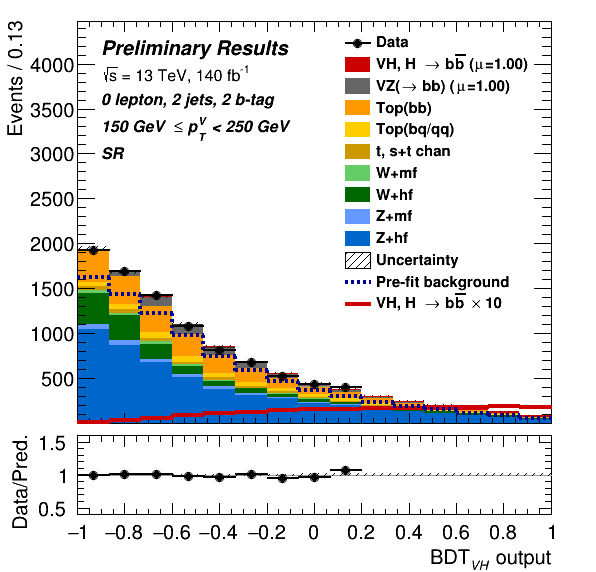
\includegraphics[width=\textwidth]{Images/VH/Own_fit/postfit_VHbb/Region_distmva_BMax250_BMin150_DSR_J2_TTypebb_T2_L0_Y6051_GlobalFit_conditionnal_mu1.png}
        \caption{0L, 2-jet 150 GeV $<$ \ptv\ $<$ 250 GeV $BB$-tagged.}
        \label{fig:posfit_0L_SR}
    \end{subfigure}
    \begin{subfigure}[b]{0.32\textwidth}
        \centering
        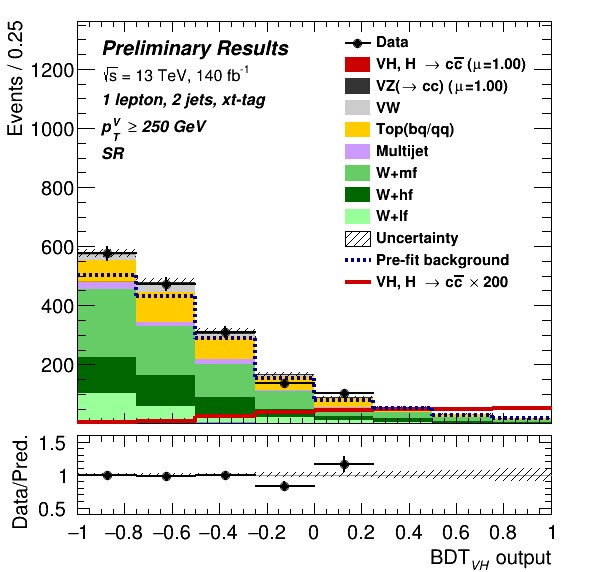
\includegraphics[width=\textwidth]{Images/VH/Own_fit/postfit_VHcc/Region_distmva_BMin250_DSR_J2_TTypext_T2_L1_Y6051_GlobalFit_conditionnal_mu1.png}
        \caption{1L, 2-jet \ptv\ $>$ 250 GeV 2 $c$-tagged.}
        \label{fig:posfit_1L_SR}
    \end{subfigure}
    \begin{subfigure}[b]{0.32\textwidth}
      \centering
      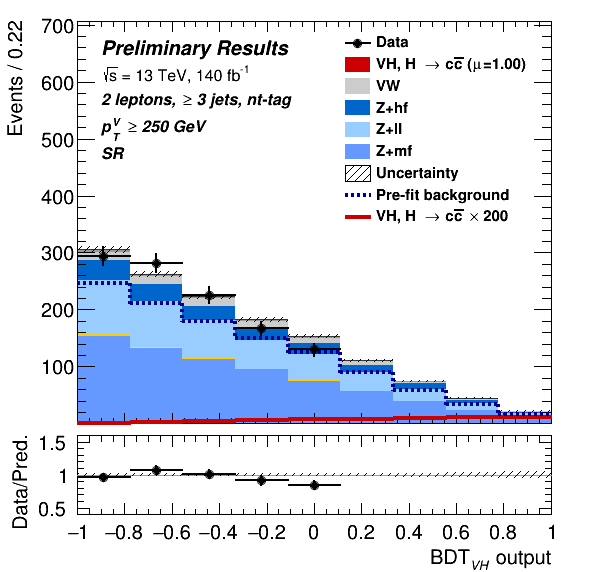
\includegraphics[width=\textwidth]{Images/VH/Own_fit/postfit_VHcc/Region_distmva_BMin250_DSR_J3_TTypent_incJet1_T1_L2_Y6051_GlobalFit_conditionnal_mu1.png}
      \caption{2L, $\geq$3-jet \ptv\ $>$ 250 GeV 1 $c$-tagged.}
      \label{fig:posfit_2L_SR}
    \end{subfigure} \\
    \begin{subfigure}[b]{0.32\textwidth}
        \centering
        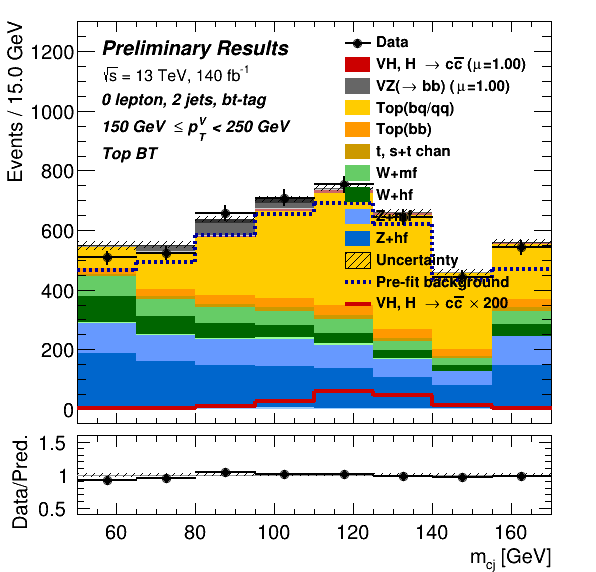
\includegraphics[width=\textwidth]{Images/VH/Own_fit/postfit_VHcc/Region_distmBB_BMax250_BMin150_DtopCRBC_J2_TTypebt_T1_L0_Y6051_GlobalFit_conditionnal_mu1.png}
        \caption{0L, 2-jet 150 GeV $<$ \ptv\ $<$ 250 GeV Top $BT$ CR.}
        \label{fig:posfit_0L_CR}
    \end{subfigure}
    \begin{subfigure}[b]{0.32\textwidth}
        \centering
        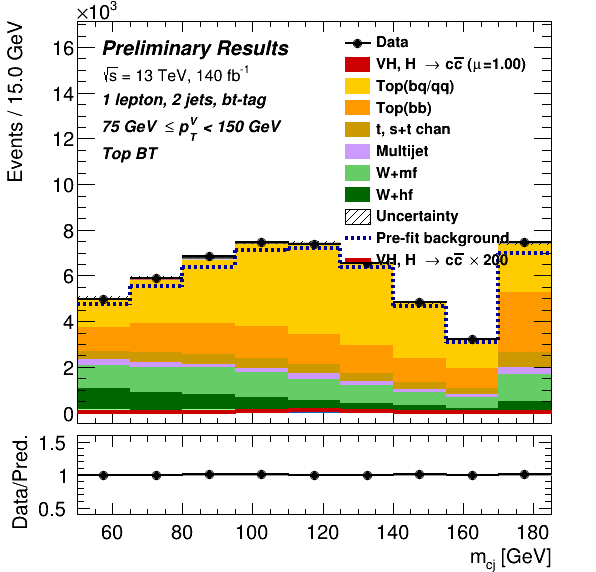
\includegraphics[width=\textwidth]{Images/VH/Own_fit/postfit_VHcc/Region_distmBB_BMax150_BMin75_DtopCRBC_J2_TTypebt_T1_L1_Y6051_GlobalFit_conditionnal_mu1.png}
        \caption{1L, 2-jet 75 GeV $<$ \ptv\ $<$ 150 GeV Top $BT$ CR.}
        \label{fig:posfit_1L_CR}
    \end{subfigure}
    \begin{subfigure}[b]{0.32\textwidth}
        \centering
        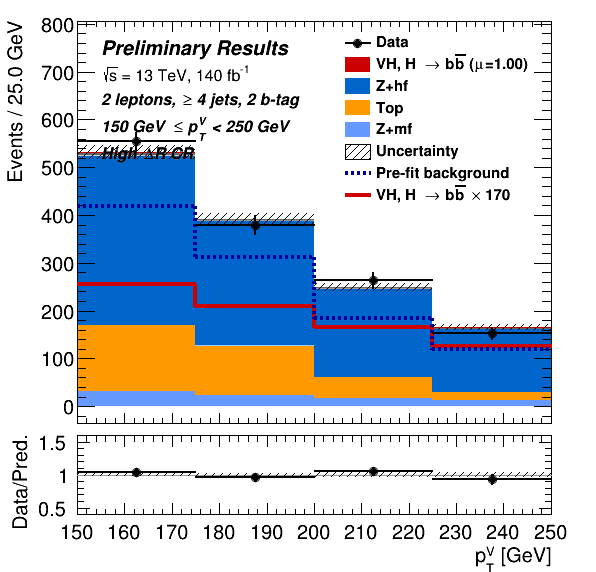
\includegraphics[width=\textwidth]{Images/VH/Own_fit/postfit_VHbb/Region_distpTV_BMax250_BMin150_DCRHigh_J4_TTypebb_incJet1_T2_L2_Y6051_GlobalFit_conditionnal_mu1.png}
        \caption{2L, $\geq$ 4-jet 250 GeV $<$ \ptv\ $<$ 400 GeV $BB$-tagged CRHigh.}
        \label{fig:posfit_2L_CR}
    \end{subfigure}
    \caption{Selected posfit signal regions (top row) and control regions (bottom row), for the 0L (left), 1L (centre), and 2L (right).}
    \label{fig:postfit_SR_CR}
\end{figure} 

\begin{figure}[h!]
    \centering
    \begin{subfigure}[b]{0.32\textwidth}
        \centering
        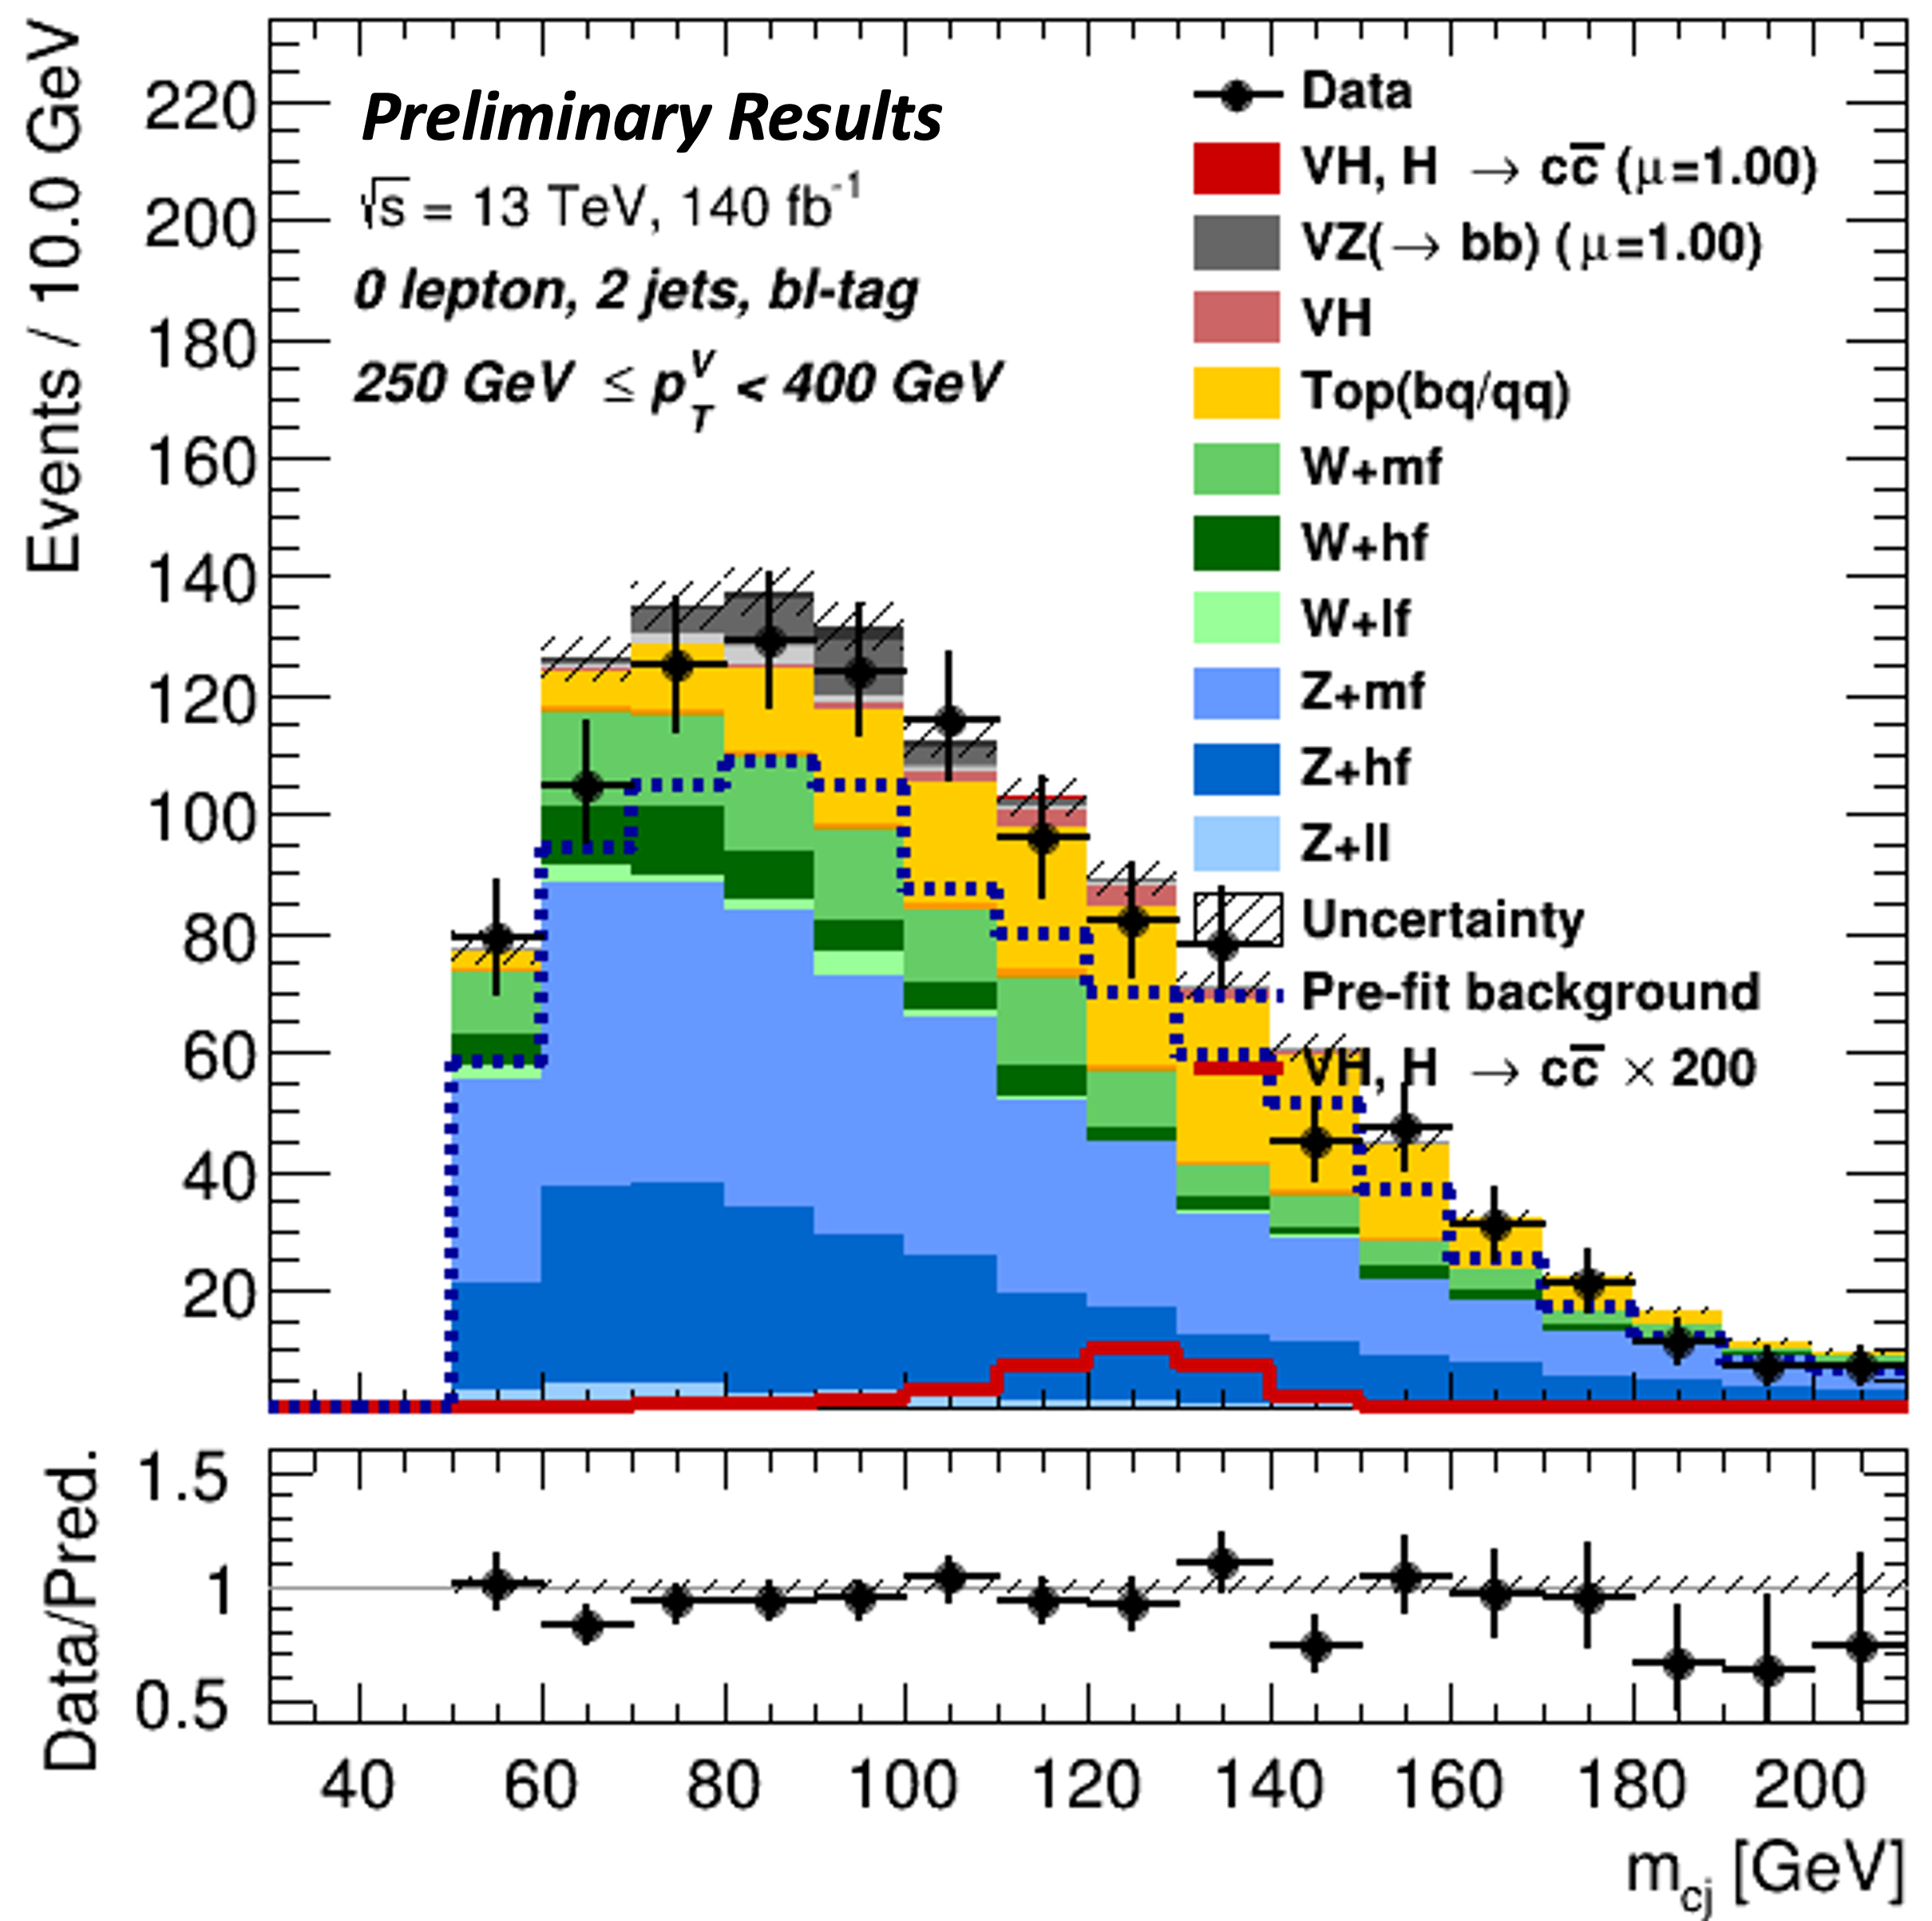
\includegraphics[width=\textwidth]{Images/VH/Fit/fromSlides/Postfit/0LtopCRBL.png}
        \caption{0L $BL$-tagged, Top $BT$ CR-like.}
        \label{fig:val_BLtopCR}
    \end{subfigure}
    \begin{subfigure}[b]{0.32\textwidth}
        \centering
        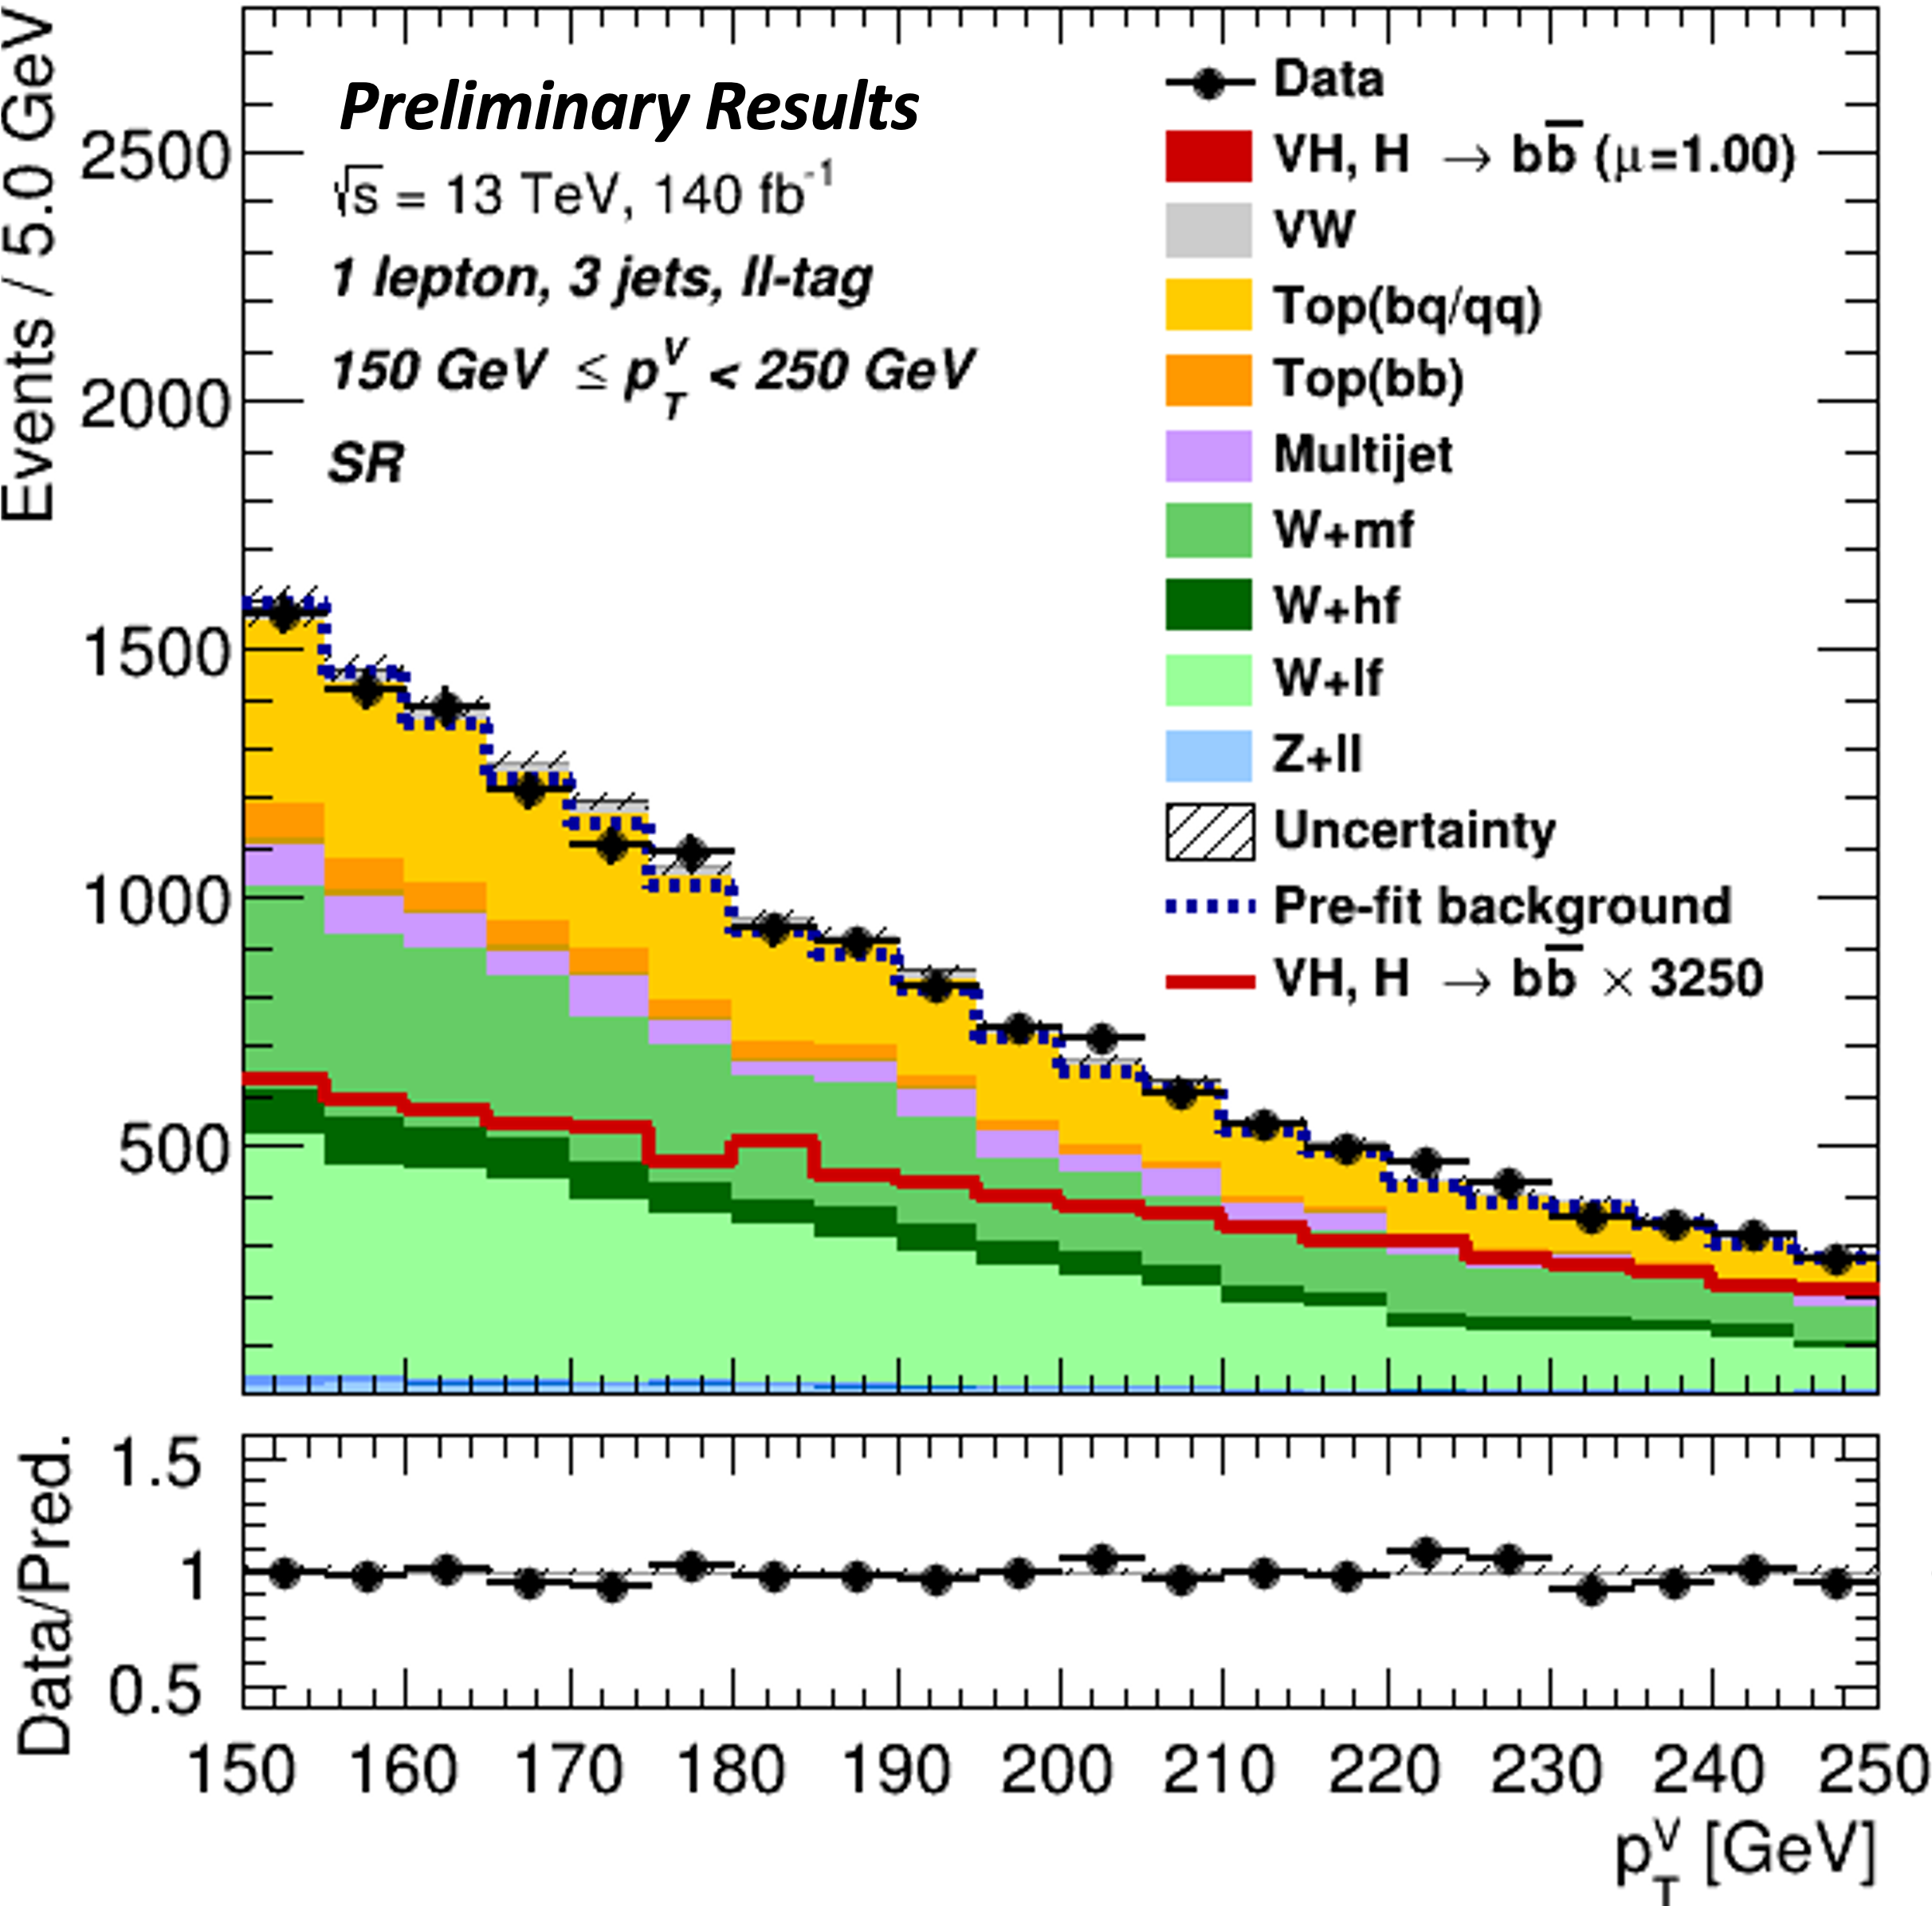
\includegraphics[width=\textwidth]{Images/VH/Fit/fromSlides/Postfit/1L_LLSR.png}
        \caption{1L $LL$, $c$-tagged SR-like.}
        \label{fig:val_LLSR}
    \end{subfigure}
    \begin{subfigure}[b]{0.32\textwidth}
      \centering
      \includegraphics[width=\textwidth]{Images/VH/Fit/fromSlides/Postfit/2LBB.png}
      \caption{2L \ptv\ in 2-jets $BB$ SR.}
      \label{fig:fit_ptv2L}
    \end{subfigure} 
    \caption{Posfit distributions in a $BL$-tagged Top CR-like (left) and $LL$-tagged SR-like (centre) validations regions and the 2L \ptv\ spectrum in the 2-jet $BB$-tagged SR.}
    \label{fig:postfitval}
\end{figure} 


The breakdown of the uncertainties, presented in Table \ref{tab:exp-breakdown}, is a measure of the different contributions of the uncertainties to the \vhbc\ analysis. The \gls{np}s are grouped based on their origin, and their impact on the signal strengths of \vhb\ and \vhc\ is assessed by iteratively re-running fits with successive groups of \gls{np}s fixed at their postfit values. The notation adopted is to label the signal strengths (one for \vhb\ and one for \vhc) of the nominal maximal likelihood fit as $\hat{\mu}$ with uncertainty $\sigma_{\hat{\mu}}$, and of a re-ran fit with a group of \gls{np}s fixed as $\hat{\mu}'$ with uncertainty $\sigma_{\hat{\mu}'}$. The impact of the fixed group of \gls{np}s is defined as the change in uncertainty measured by 
\begin{equation}
    \text{Impact} = \sqrt{\sigma^2_{\hat{\mu}} - \sigma^2_{\hat{\mu'}}}.
\end{equation}

\begin{table}[h!]
    \centering
    \renewcommand*{\arraystretch}{1.3}
    \begin{tabular}{l  C{2cm} C{2cm}}
        \hline \hline
        Source of Uncertainty & $\mu_{VH(H\rightarrow b\bar{b})}$ & $\mu_{VH(H\rightarrow c\bar{c})}$ \\
        \hline
        \textbf{Total}               &  0.127 & 5.089 \\
        \textbf{Statistics}          &  0.095 & 3.791 \\
        \textbf{Systematics }        &  0.085 & 3.395 \\ 
        \hline \hline
        \textbf{Statistical Uncertainties} & 0.095 & 3.791 \\
        Data sample size             &  0.088 & 3.538 \\
        Floating normalisations      &  0.029 & 1.247 \\
        Top $e\mu$ CR statistics     &  0.011 & 0.130 \\ 
        \hline \hline
        \textbf{Systematics Uncertainties} & 0.085 & 3.395 \\ 
        \vhbc\ Modelling         & 0.021 & 0.237 \\
        \hline
        \textbf{Backgrounds Modelling}    & 0.069 & 2.739 \\
        $Z+$jets                     &  0.036 & 1.587 \\
        $W+$jets                     &  0.036 & 1.088 \\
        Diboson                      &  0.020 & 0.546 \\
        \ttb\                        &  0.011 & 0.613 \\
        single-top                   &  0.008 & 0.116 \\
        Multi-jet                    &  0.007 & 0.691 \\
        \hline
        \textbf{Experimental Uncertainties} & 0.035 & 1.278 \\
        Jet                          &  0.026 & 0.737 \\
        Large-$R$ jet                &  0.009 & 0.206 \\
        \etm\                        &  0.007 & 0.150 \\
        Lepton                       &  0.004 & 0.115 \\
        FTAG PFlow ($b$-jet)         &  0.015 & 0.258 \\
        FTAG PFlow ($c$-jet)         &  0.008 & 0.769 \\
        FTAG PFlow (light-jet)         &  0.003 & 0.751 \\
        FTAG PFlow (extrap)          &  0.000 & 0.000 \\
        FTAG VR ($b$-jet)            &  0.004 & 0.049 \\
        FTAG VR ($c$-jet)            &  0.001 & 0.018 \\
        FTAG VR (light-jet)            &  0.001 & 0.009 \\
        FTAG VR (extrap)             &  0.001 & 0.037 \\
        Pile-up                      &  0.005 & 0.052 \\
        Luminosity                   &  0.007 & 0.035 \\
        \hline
        \textbf{MC-samples Size}     &  0.020 & 1.410 \\
        \hline \hline
    \end{tabular}
    \caption{Breakdown of the different systematics and statistical uncertainties.}
    \label{tab:exp-breakdown}
\end{table}

To define the impact of the statistical uncertainties, a fit is run with all \gls{np}s fixed except for the floating normalisations. The total systematics effect is set to the difference in quadrature between the total and the statistical uncertainties. For both the \vhb\ and \vhc\ measurements, the statistical and systematic uncertainties are of similar size, with the statistical uncertainties being slightly larger. The uncertainties are far smaller for the \vhb\ side, as expected from the larger statistics and better performance of both the experimental reconstruction and modelling. For \vhb, the largest contributions to the systematics uncertainties come from the $V+$jets and diboson background modelling, and the signal modelling. The importance of the $V+$jets is expected since the $W+$jets and $Z+$jets play a significant role in the 1-lepton and the 0- and 2-lepton channels respectively. On the experimental side, the jet and flavour tagging uncertainties are leading. For the latter, the $b$-jets uncertainties contribute the most followed by the $c$-jets, as expected from the resemblance between heavy flavour jet species. \\

For \vhc, similar observations can be made with several nuances. On the modelling side, the signal modelling is less paramount, with the top processes and multi-jet not contributing far more significantly. Additionally, the $Z+$jets uncertainties are now clearly the leading one, with the $W+$jets proportionally less important. This latter observation is connected with the larger importance of the top processes, as \vhc\ has a much larger top contribution in the 1-lepton channel, competing with $W+$jets as the leading source of uncertainty there. On the experimental side, the flavour tagging uncertainties of the $c$- and light-jet are now dominant, with the jet uncertainties. This is expected from the challenges of tagging and reconstructing $c$-jets. The statistic of the \gls{mc}-samples is far more important on the \vhc\ side, mostly due to the low $c$-tagging efficiency of the \gls{dl1r} tagger used. \\

A second technique to assess the importance of different nuisance parameters on the signal strengths is to change their \gls{np} values upwards and downwards by their postfit uncertainties $\sigma_{\theta}$ and re-run the fit with the modified \gls{np} fixed. For each \gls{np}, this requires running two fits in addition to the nominal fit from which $\hat{\theta}$ and $\sigma_{\hat{\theta}}$ are measured: one with the \gls{np} fixed at $\hat{\theta} + \sigma_{\hat{\theta}}$ and one with $\hat{\theta} - \sigma_{\hat{\theta}}$. \gls{np}s are ranked by the difference in the signal strengths between these new fits and the nominal one, as shown in Figure \ref{fig:rankingPostfit}. In these plots, the central values of \gls{np}s are set at 0 (1 for \gls{fn}s and $\gamma$-factor) as the dataset is the postfit Asimov set. For \vhb, the \whf\ extrapolations have a significant impact on the predicted signal strength, with several of these systematics highly ranked. Shape uncertainties associated with the diboson process and Higgs modelling uncertainties as well as the $Wt$ DS-DR shape uncertainty and a $b$-jet tagging uncertainty also contribute meaningfully. The floating normalisation of \whf\ in the boosted region is the only \gls{fn} to make the ranking, due to its significant pull as is shown below in Figure \ref{fig:FNback}. For \vhc, the Top process \gls{carl} shapes are the leading nuisance parameters, with the $Z+cc$ shape and the $W+$jets $cc/bb$ acceptance ratio. The \zlf\ and, to a lesser extent, \wlf\ floating normalisations have a large impact on the predicted signal strength, despite the constraints offered by the $V+l$ \gls{cr}. The light- and $c$-jets uncertainties from flavour tagging are the biggest contributors in this category. Finally, the multi-jet process normalisation enters the ranking as this process contributes more in \vhc. The $\gamma$-factor listed corresponds to the last unblinded bin in the 1L high \ptv\ 2-jet \gls{sr}, shown in Figure \ref{fig:posfit_1L_SR}, where a large amount of signal is expected, and the effect of this \gls{np} should be reduced once the signal is no longer constrained to its \gls{sm} expectations in a conditional data fit.

\begin{figure}[h!]
    \centering
    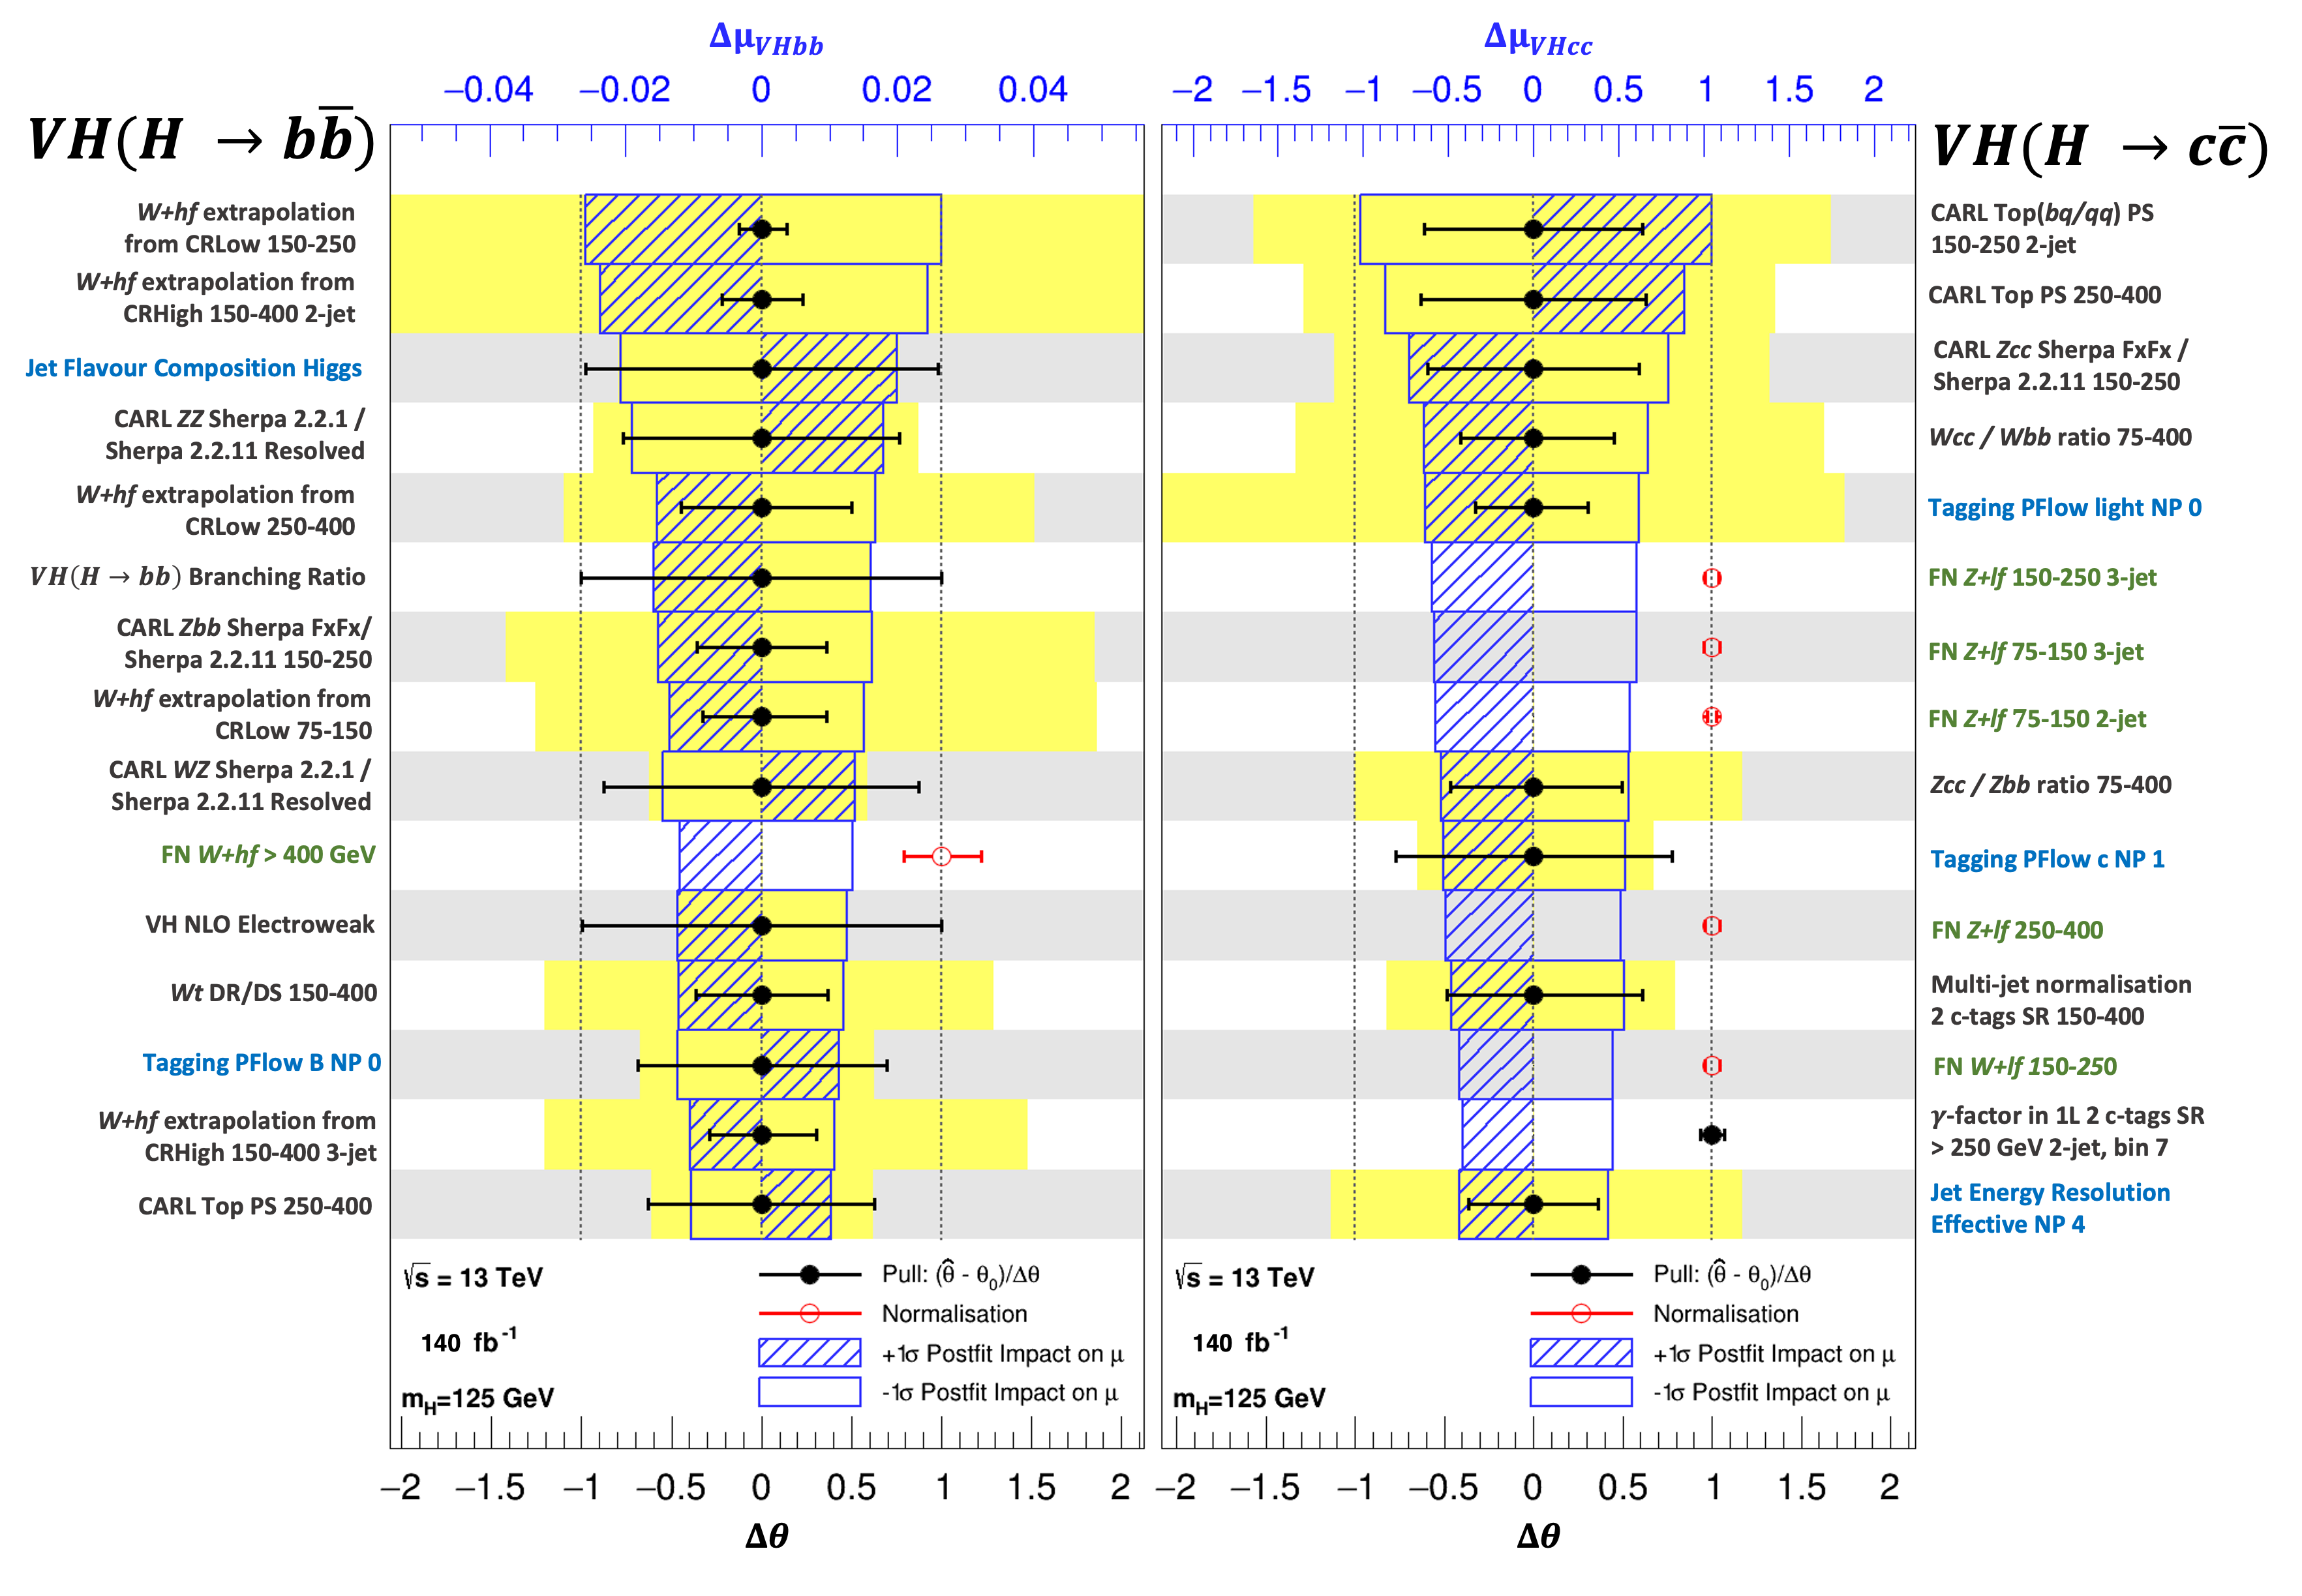
\includegraphics[width=\textwidth]{Images/VH/Fit/fromSlides/ranking.png}
    \caption{The 15 most highly ranked Asimov postfit nuisance parameters for the \vhb\ (left) and \vhc\ (right) signal strengths. Modelling NPs are written in black, experimental NPs in blue, and floating normalisation (and $\gamma$-factor) in green, with values indicated by the bottom axis showing $\Delta \theta = \hat{\theta} - \theta_0$. Black points are nuisance parameters with their central value at 0 showing the pull ($\gamma$-factor with central value at 1), and red points are floating normalisation with central values at 1. The error bars on the point show the 1 $\sigma$ uncertainty of the NPs. The effect of changing the NP by +1 $\sigma$ (-1 $\sigma$) induces the change in signal strength $\Delta\mu$ shown by the hashes (empty) blue rectangle, with respect to the top axis.}
    \label{fig:rankingPostfit}
\end{figure} 

\begin{figure}[h!]
    \centering
    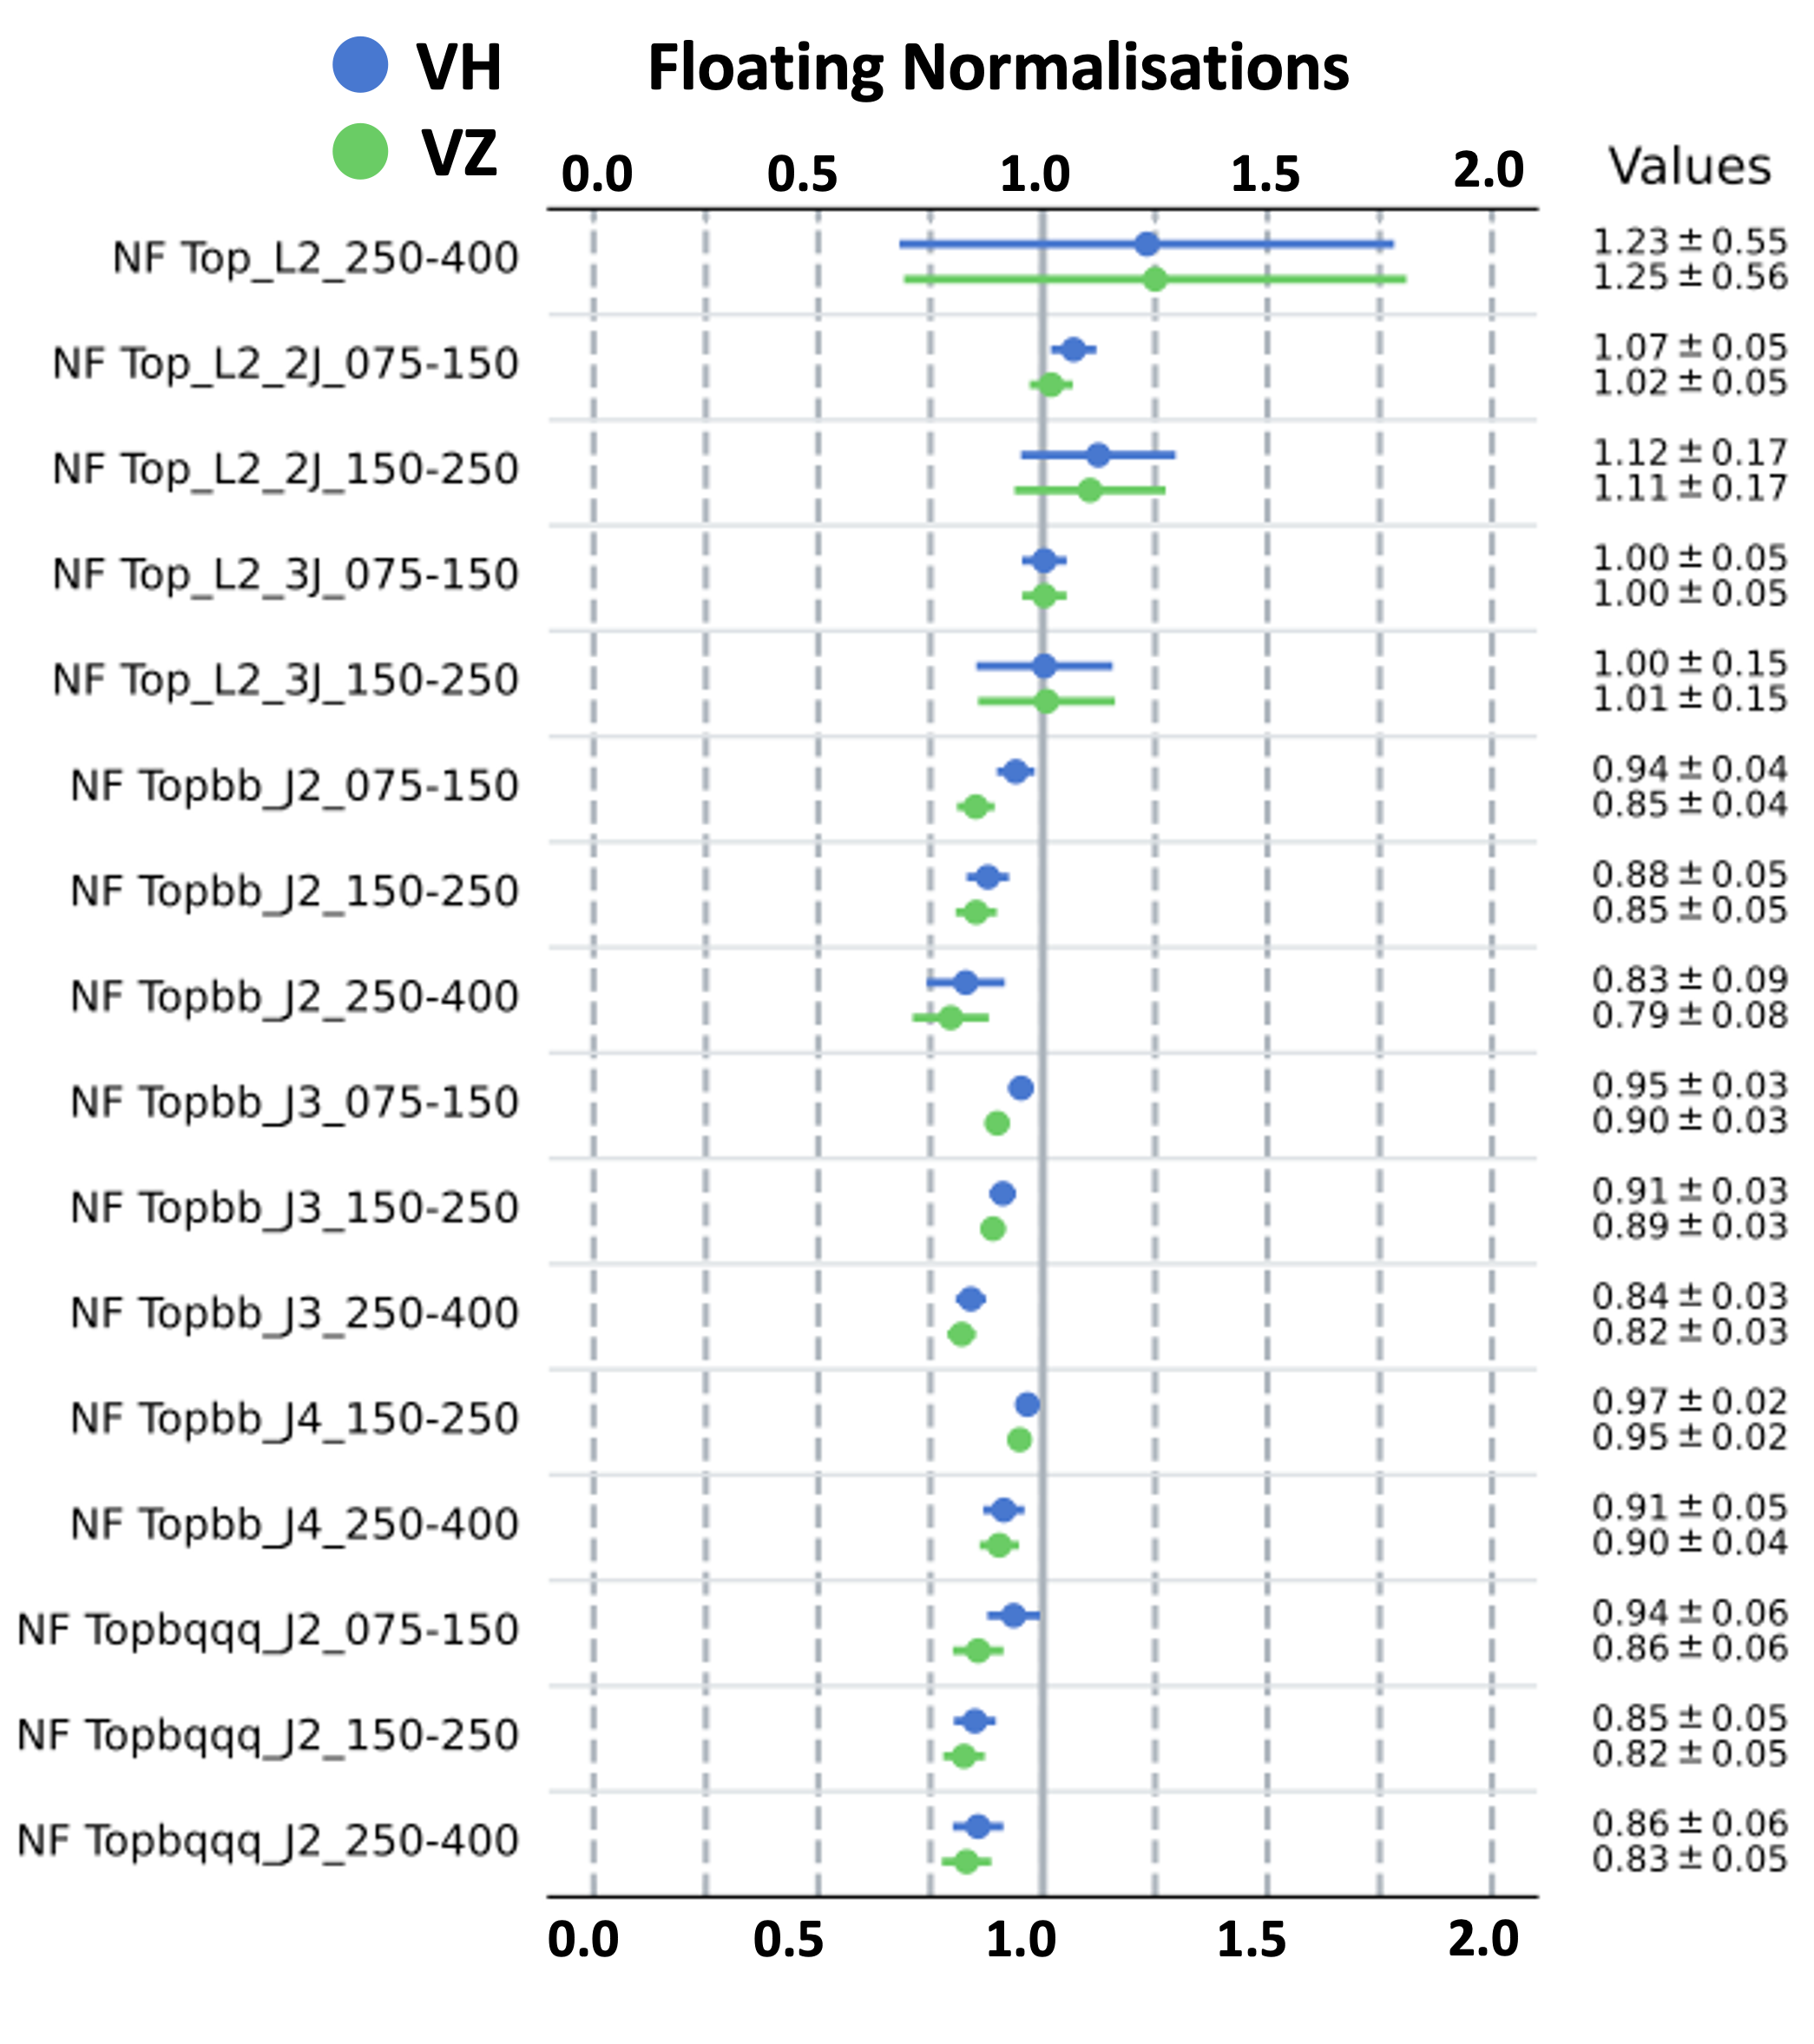
\includegraphics[width=0.48\textwidth]{Images/VH/Fit/fromSlides/FN/FN1.png}
    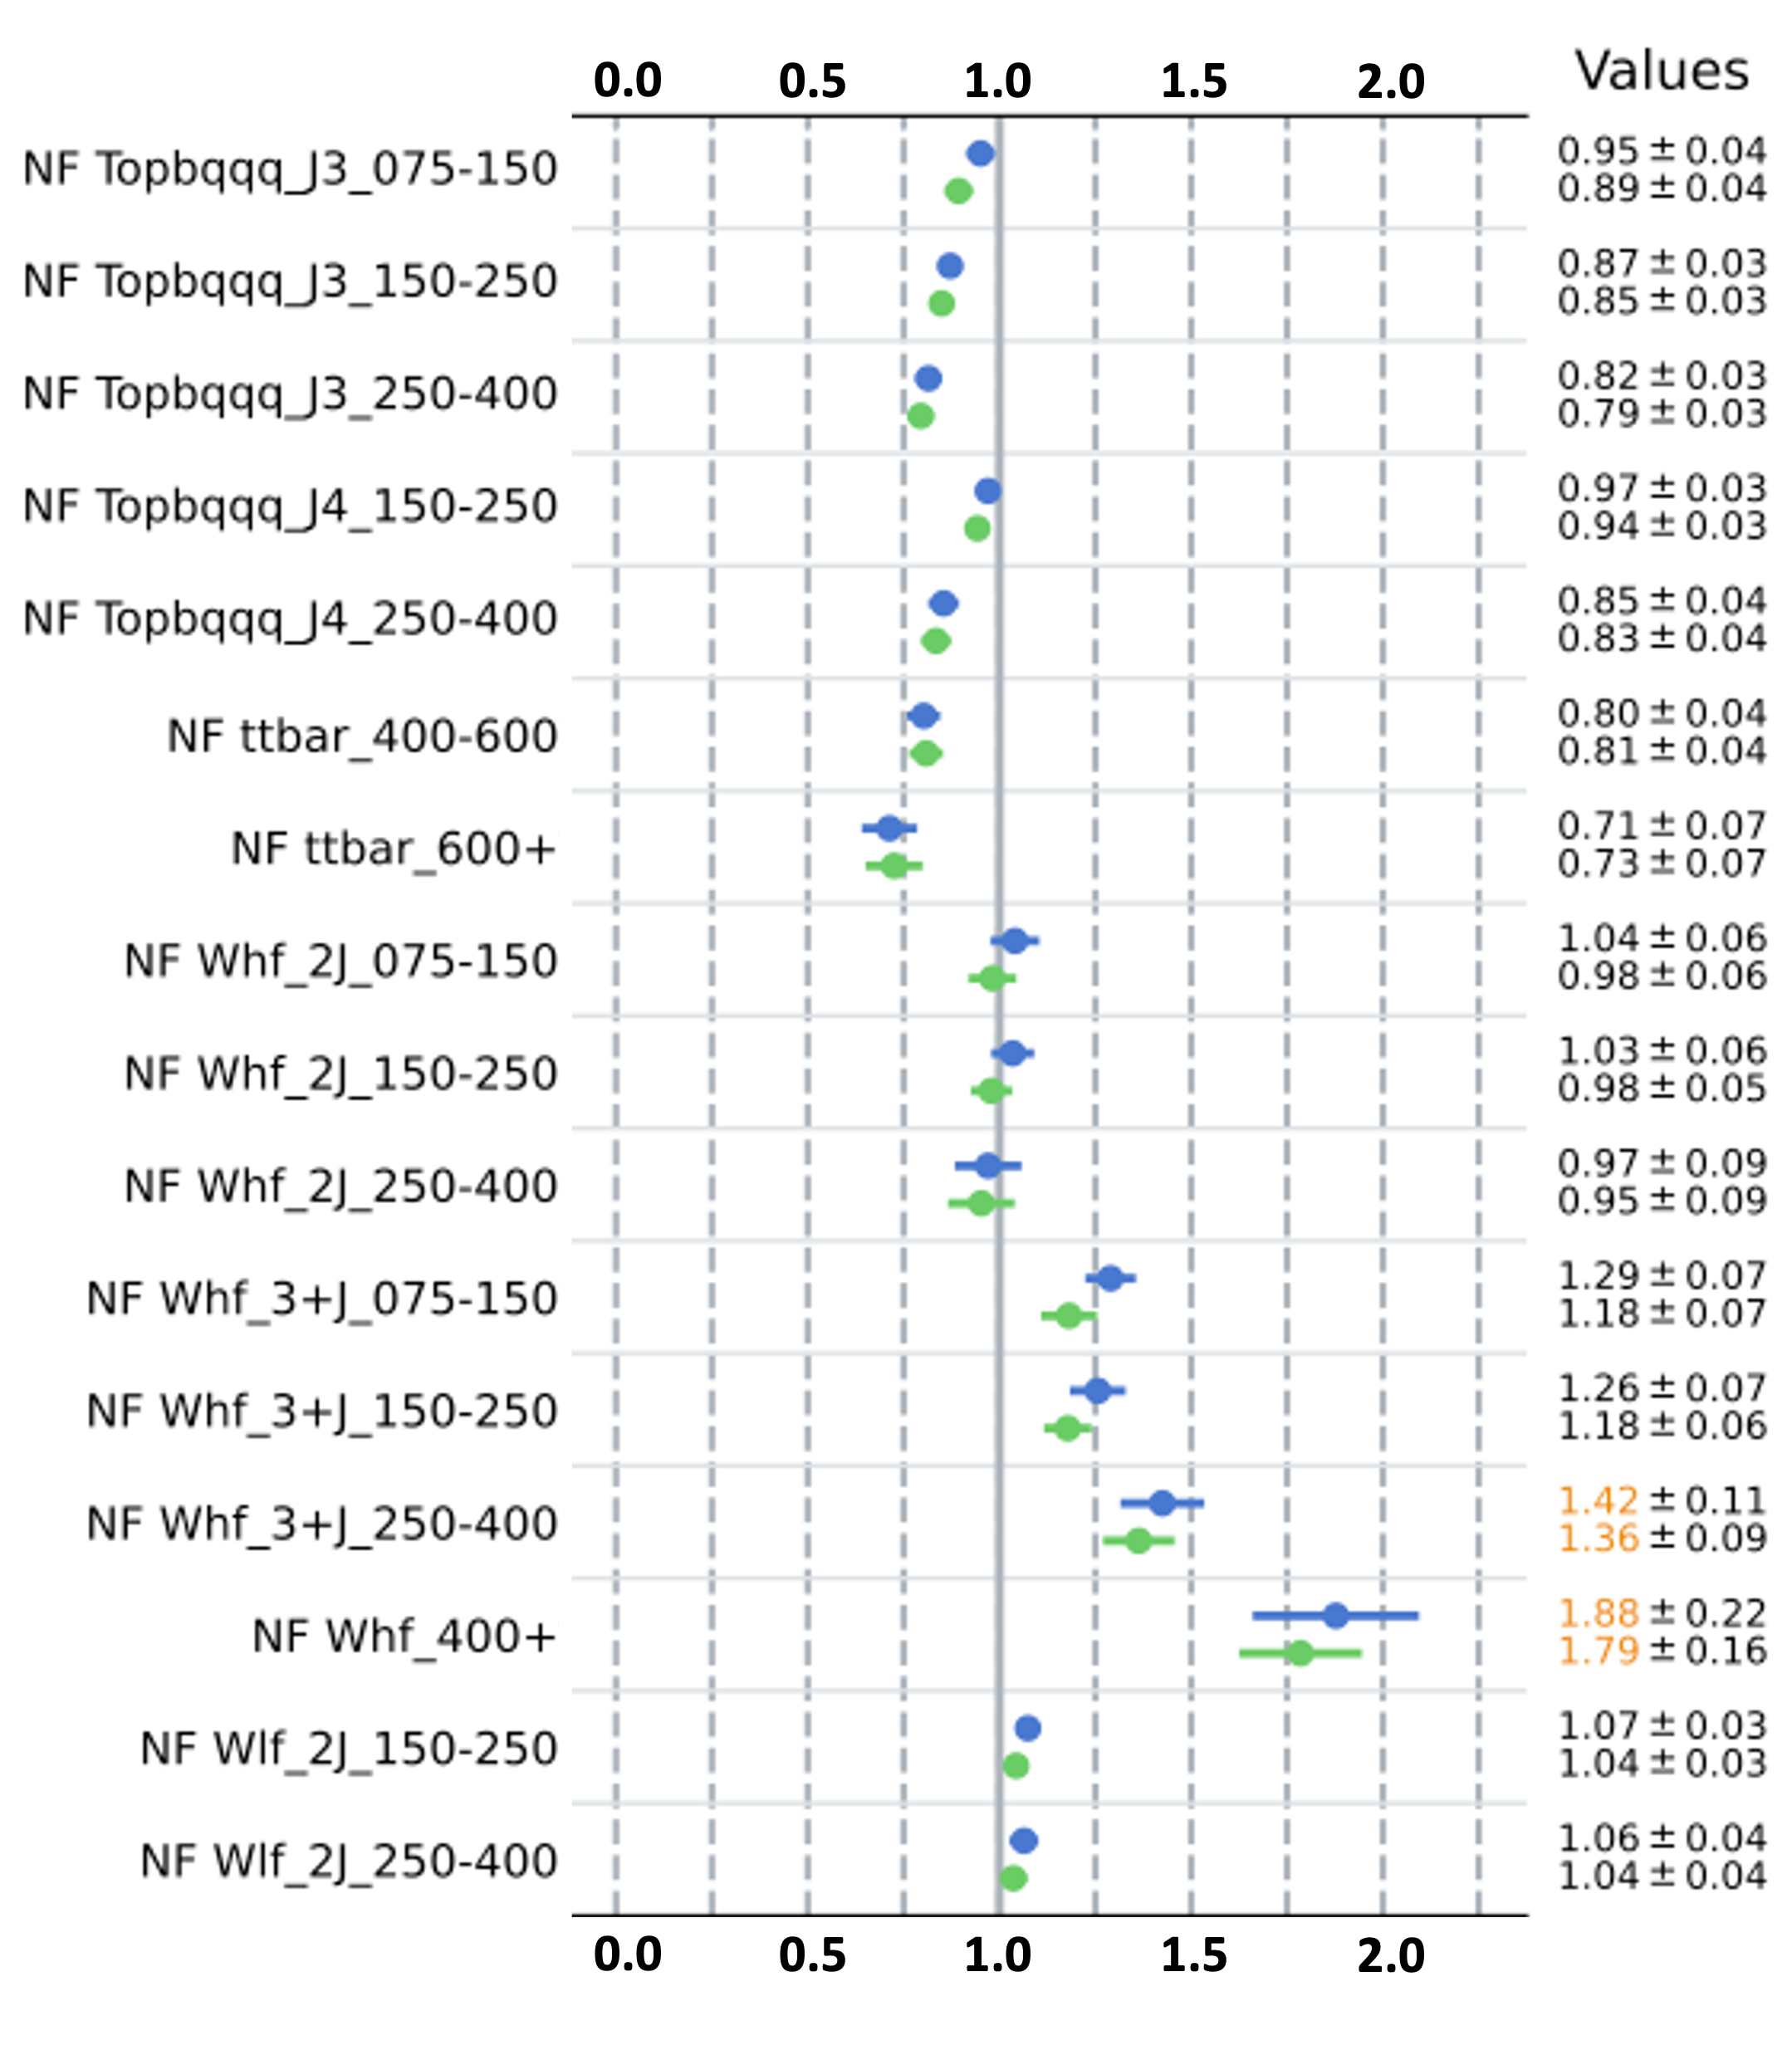
\includegraphics[width=0.48\textwidth]{Images/VH/Fit/fromSlides/FN/FN2.png}\\
    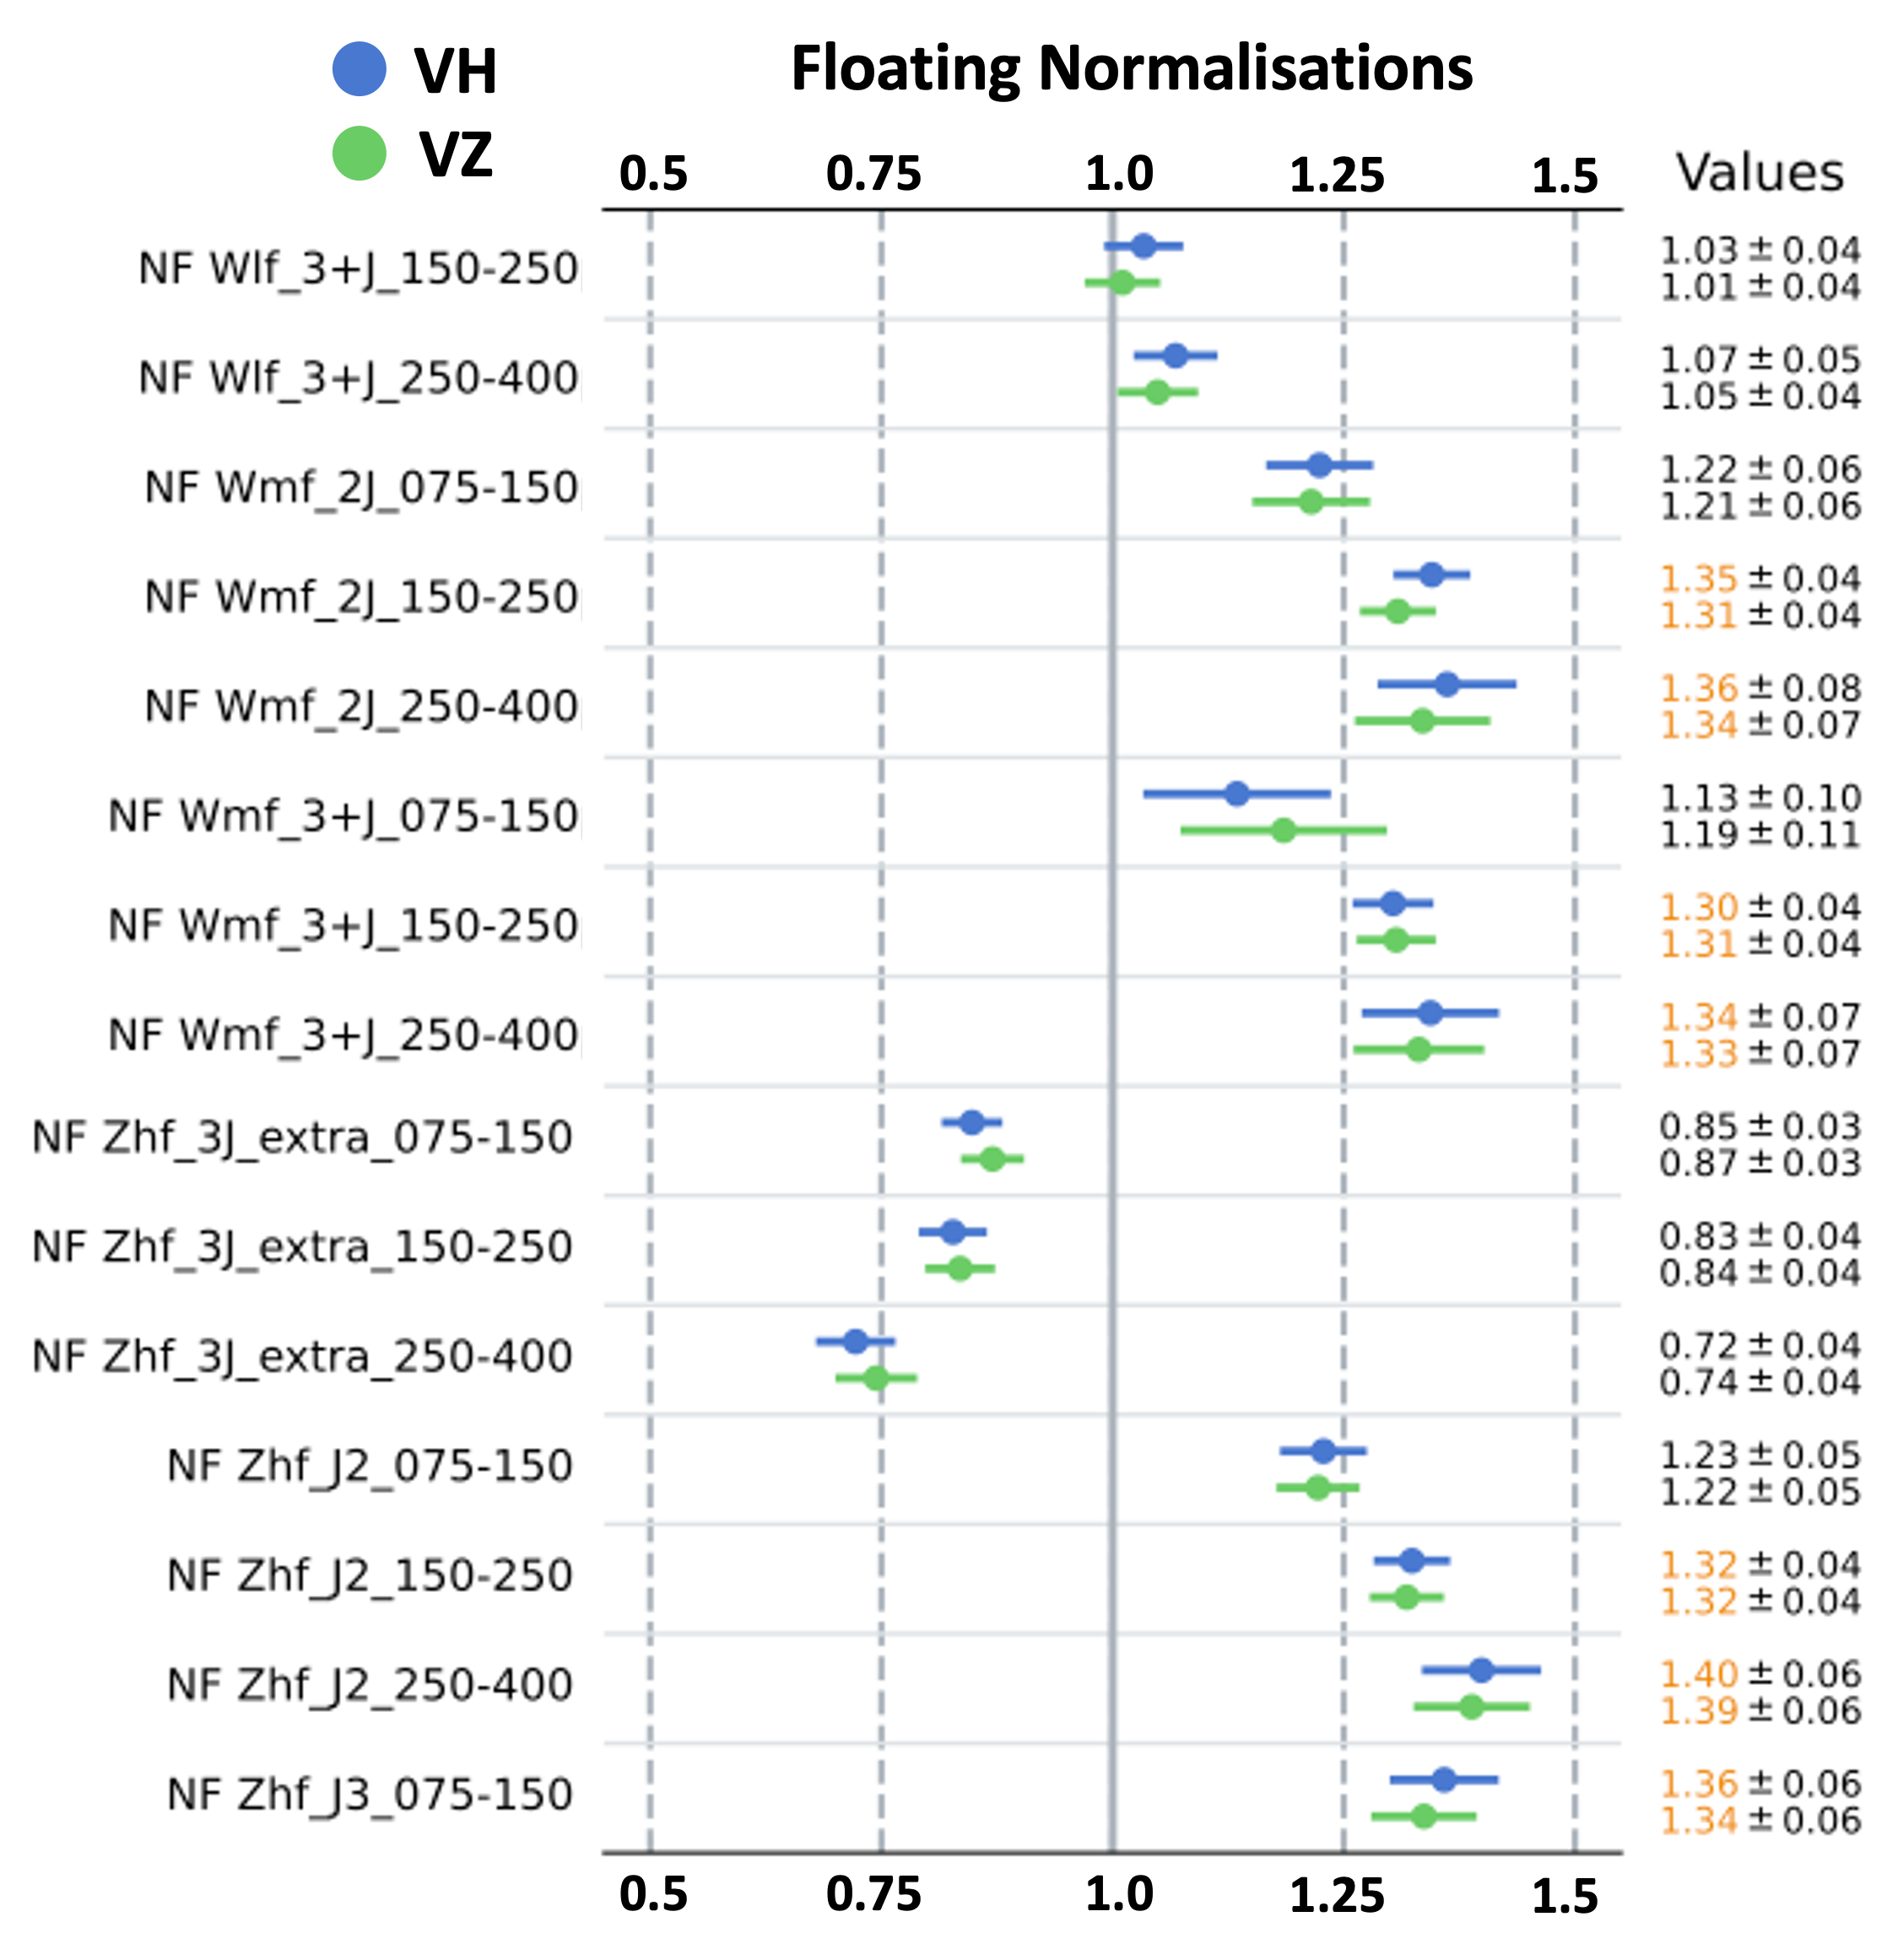
\includegraphics[width=0.48\textwidth]{Images/VH/Fit/fromSlides/FN/FN3.png}
    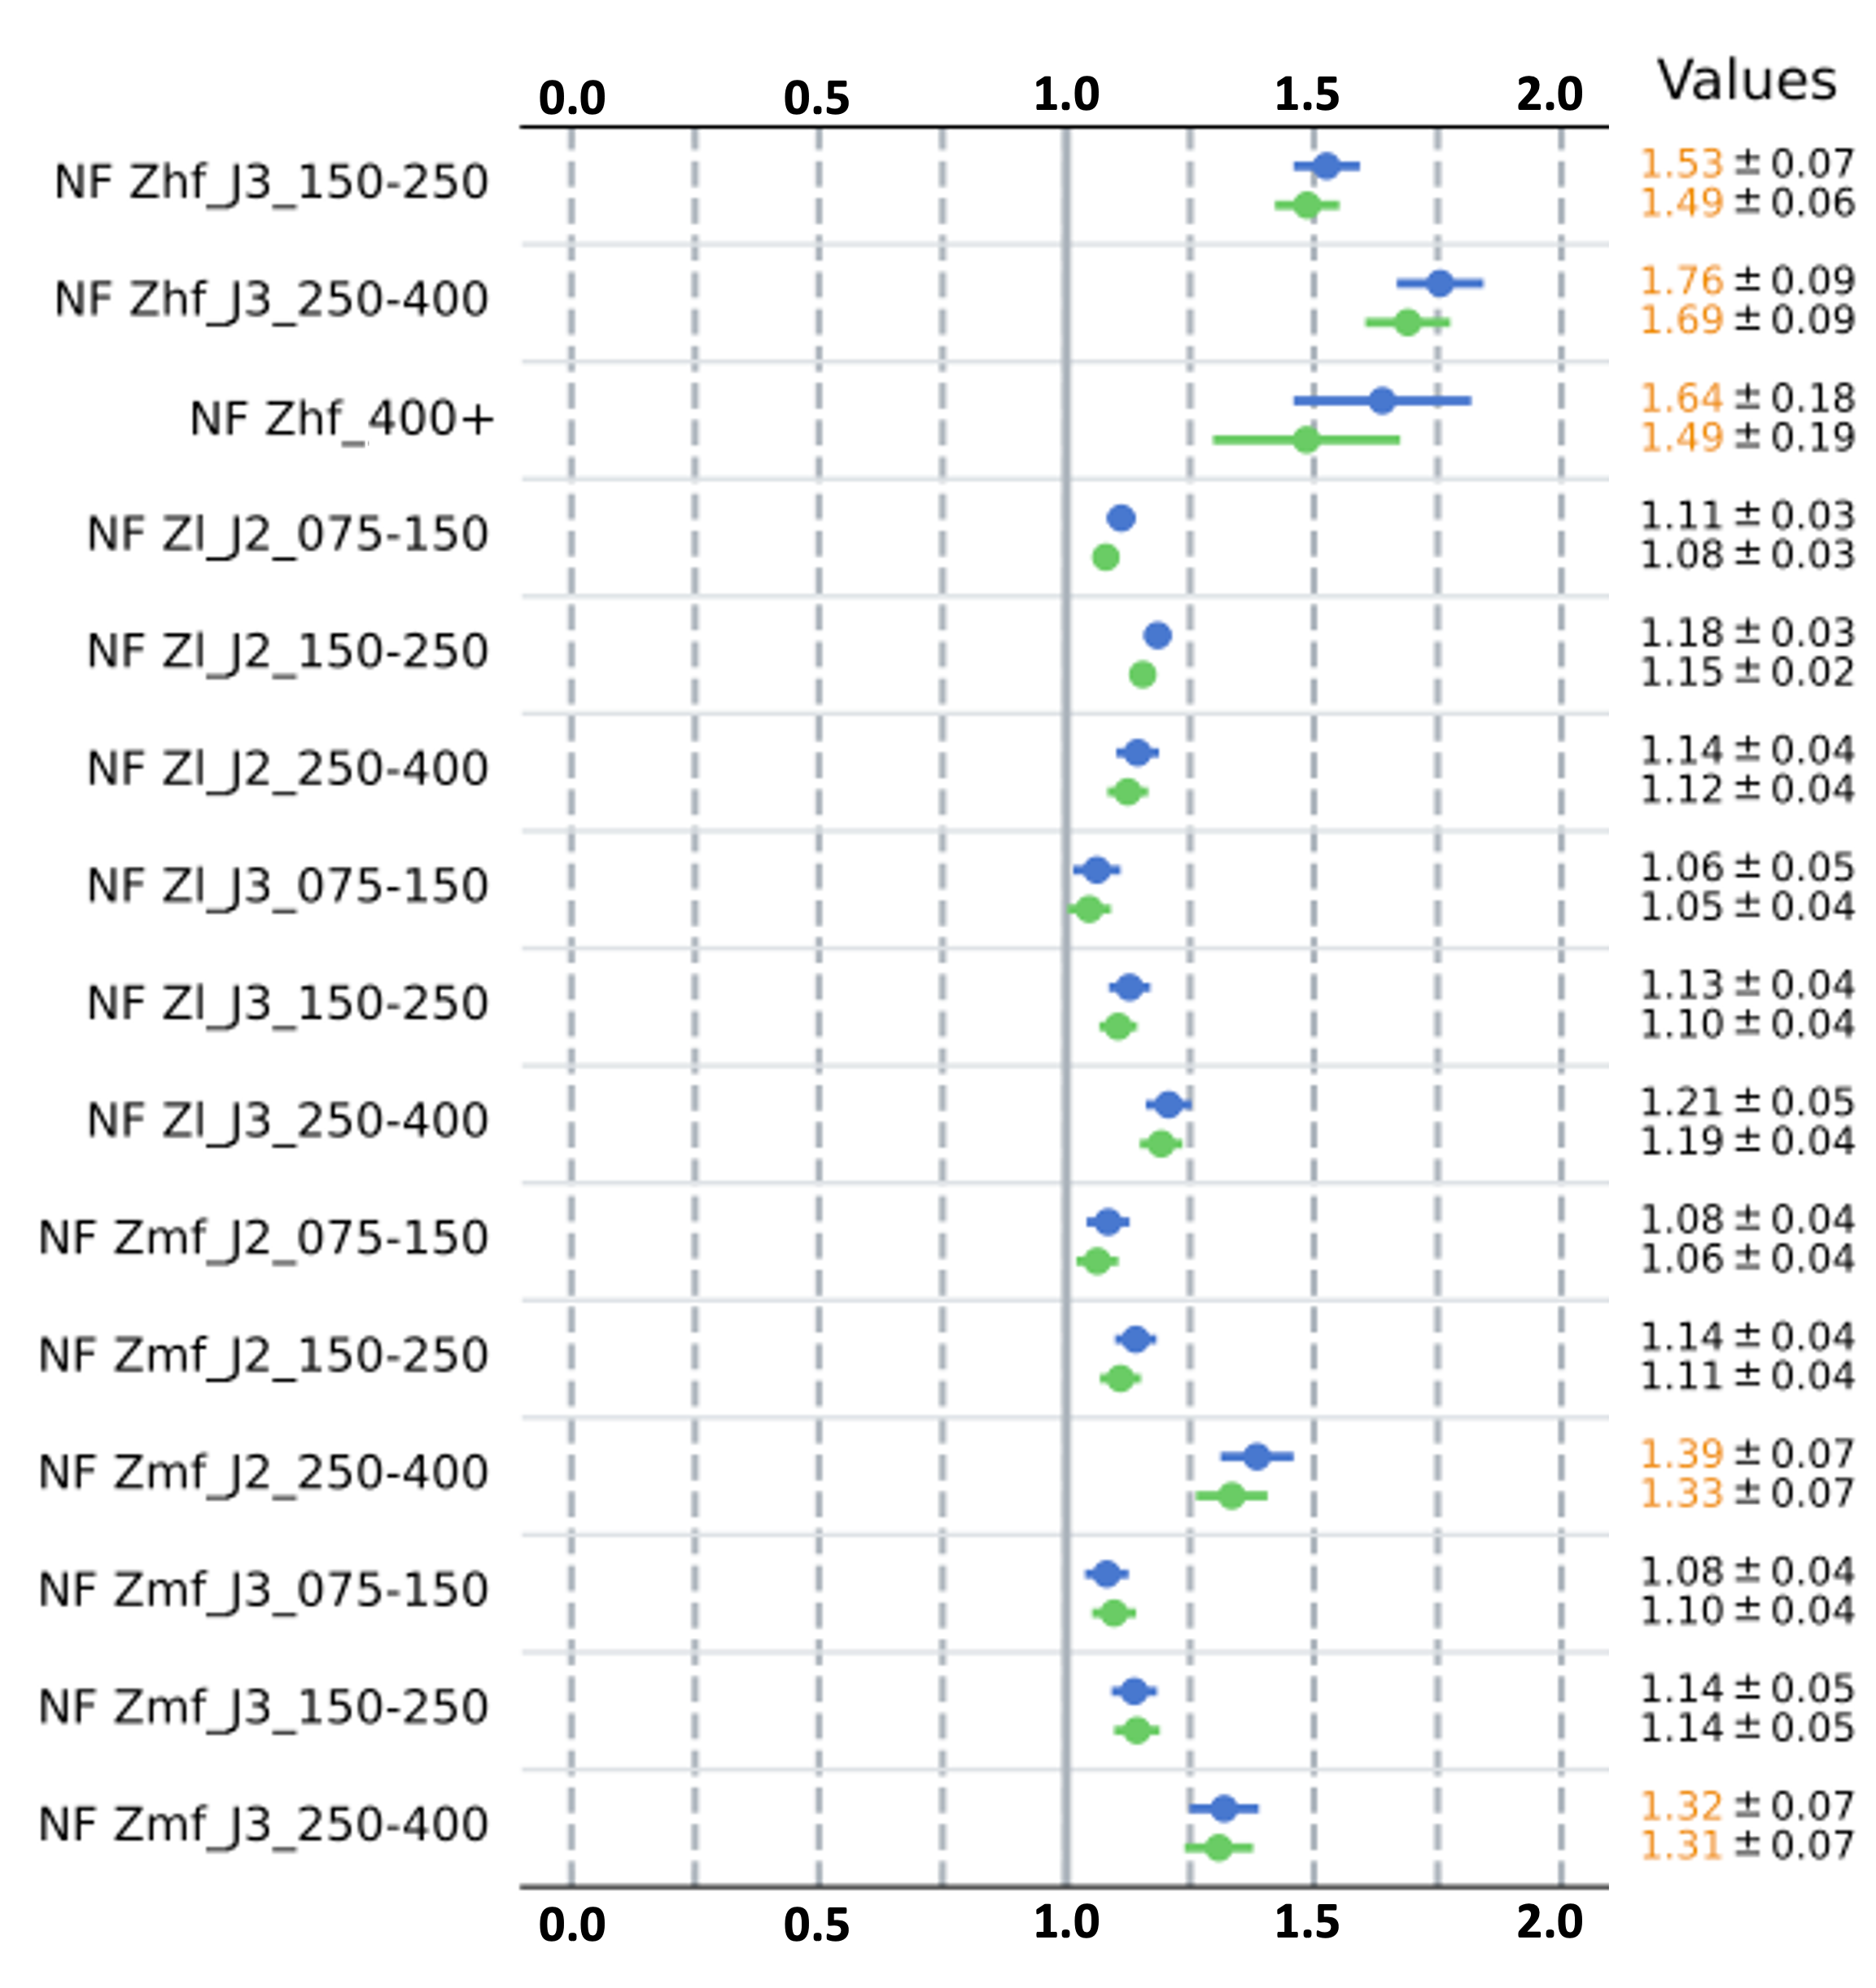
\includegraphics[width=0.48\textwidth]{Images/VH/Fit/fromSlides/FN/FN4.png}
    \caption{The floating normalisations of the major background in the combined analysis targeting the \vhbc\ in blue, versus the cross-check analysis $VZ(\rightarrow b\bar{b}/c\bar{c})$ in green.}
    \label{fig:FNback}
\end{figure} 

In the combined analysis, the major backgrounds have free-floating normalisations decorrelated across the different \ptv\ and jet multiplicity bins. The values set by a conditional likelihood fit to data, where the \vhbc\ signal strengths are set to the \gls{sm} expectations, are presented in Figure \ref{fig:FNback}. They are compared to the same \gls{fn}s obtained in the cross-check analysis with $VZ(\rightarrow b\bar{b}/c\bar{c})$ as signals. Good agreement is observed between the two sets of floating normalisations. Some common trends per process are present. Concerning the Top backgrounds, in 0L and 1L it seems mostly overestimated in the \gls{mc} simulation, with the overestimation increasing with \ptv. In 2L, the Top process seems well estimated in the Top $e\mu$ \gls{cr}, but the lower statistics available at higher \ptv\ leads to a poor constraining of the floating normalisation. The \gls{fn}s for the Top process are generally better constrained in the 3-jet than the 2-jet category, as expected from the larger yield available for this background at higher jet multiplicities. The Top$(bq/qq)$ and Top$(bb)$ have generally similar \gls{fn} values. Concerning the $W+$jets, the \whf\ is well modelled in 2-jet across \ptv\ but less so in the $\geq$3-jet category, where the underestimation of the simulations grows with \ptv. The boosted \whf\ normalisation in the $\geq$ 400 GeV range is significantly distant from 1. The same observations hold for \wlf, which is also well-modelled in 2-jet but gets higher \gls{fn}s in 3-jet. The \wmf\ component also requires large corrections from the fit, with \gls{fn} values $\sim$ 1.3 in all the \nj\ and \ptv\ bins. The final background modelled with floating normalisations is $Z+$jets, which also requires significant yield modifications from the fit in all components, jet multiplicity, and \ptv\ bins. All $Z+$jets yield are corrected up, with larger \gls{fn} values required at higher \ptv. A special case for the \zhf\ is the 3-jet and 3-jet-extra categories, adopted to account for the fact the \vhc\ side does not use 4-jet or separates 3- and $\geq$4-jet in 0L and 2L while the \vhb\ combines 3-jet with 4-jet into $\geq$3-jet in 2L. The 3-jet \gls{fn}s in the figure, labelled ``J3'', cover the $\geq$ 3-jet (for \vhb), while the 3-jet-extra, labelled ``3J\_extra'' acount only for the 3-jet category\footnote{The contribution of the \zmf\ and \zlf\ are ignored in 4-jet.}. There is therefore some overlap, with the latter set of \gls{fn}s used to correct down the large normalisation of the $\geq$ 3-jet. Similarly to the \whf, the boosted \zhf \gls{fn} value is significantly pulled away from 1.\\

The correlations between the different floating normalisations are displayed as a heat map in Figure \ref{fig:FNcorr}. A rich structure of dependencies emerges from such a plot. As expected, \gls{fn}s related to each process are highly correlated with the other \gls{fn} of the same process, in different analysis \ptv\ and \nj\ categories. Some striking exceptions are visible: the boosted \ttb\ displays a very small uncorrelation with the resolved top$(bb)$ and top$(bq/qq)$. Concerning correlations across processes, the Top$(bb)$ and Top$(bq/qq)$ are respectively seen to have large correlations with the \zhf\ (and the \whf\ in lesser extend) and the \wmf\ and \zmf, as expected from the presence of the $Z+$jets and $W$+jets in the CRHigh and the 0L and 1L $BT$-tagged Top \gls{cr}. The \whf\ normalisations are slightly anti-correlated to the \vlf and slightly correlated to the \zhf\ in the low \nj\. Similarly, the \vlf\ are strongly correlated between the $W$ and $Z$.
  
\begin{figure}[h!]
    \hspace{-1cm}
    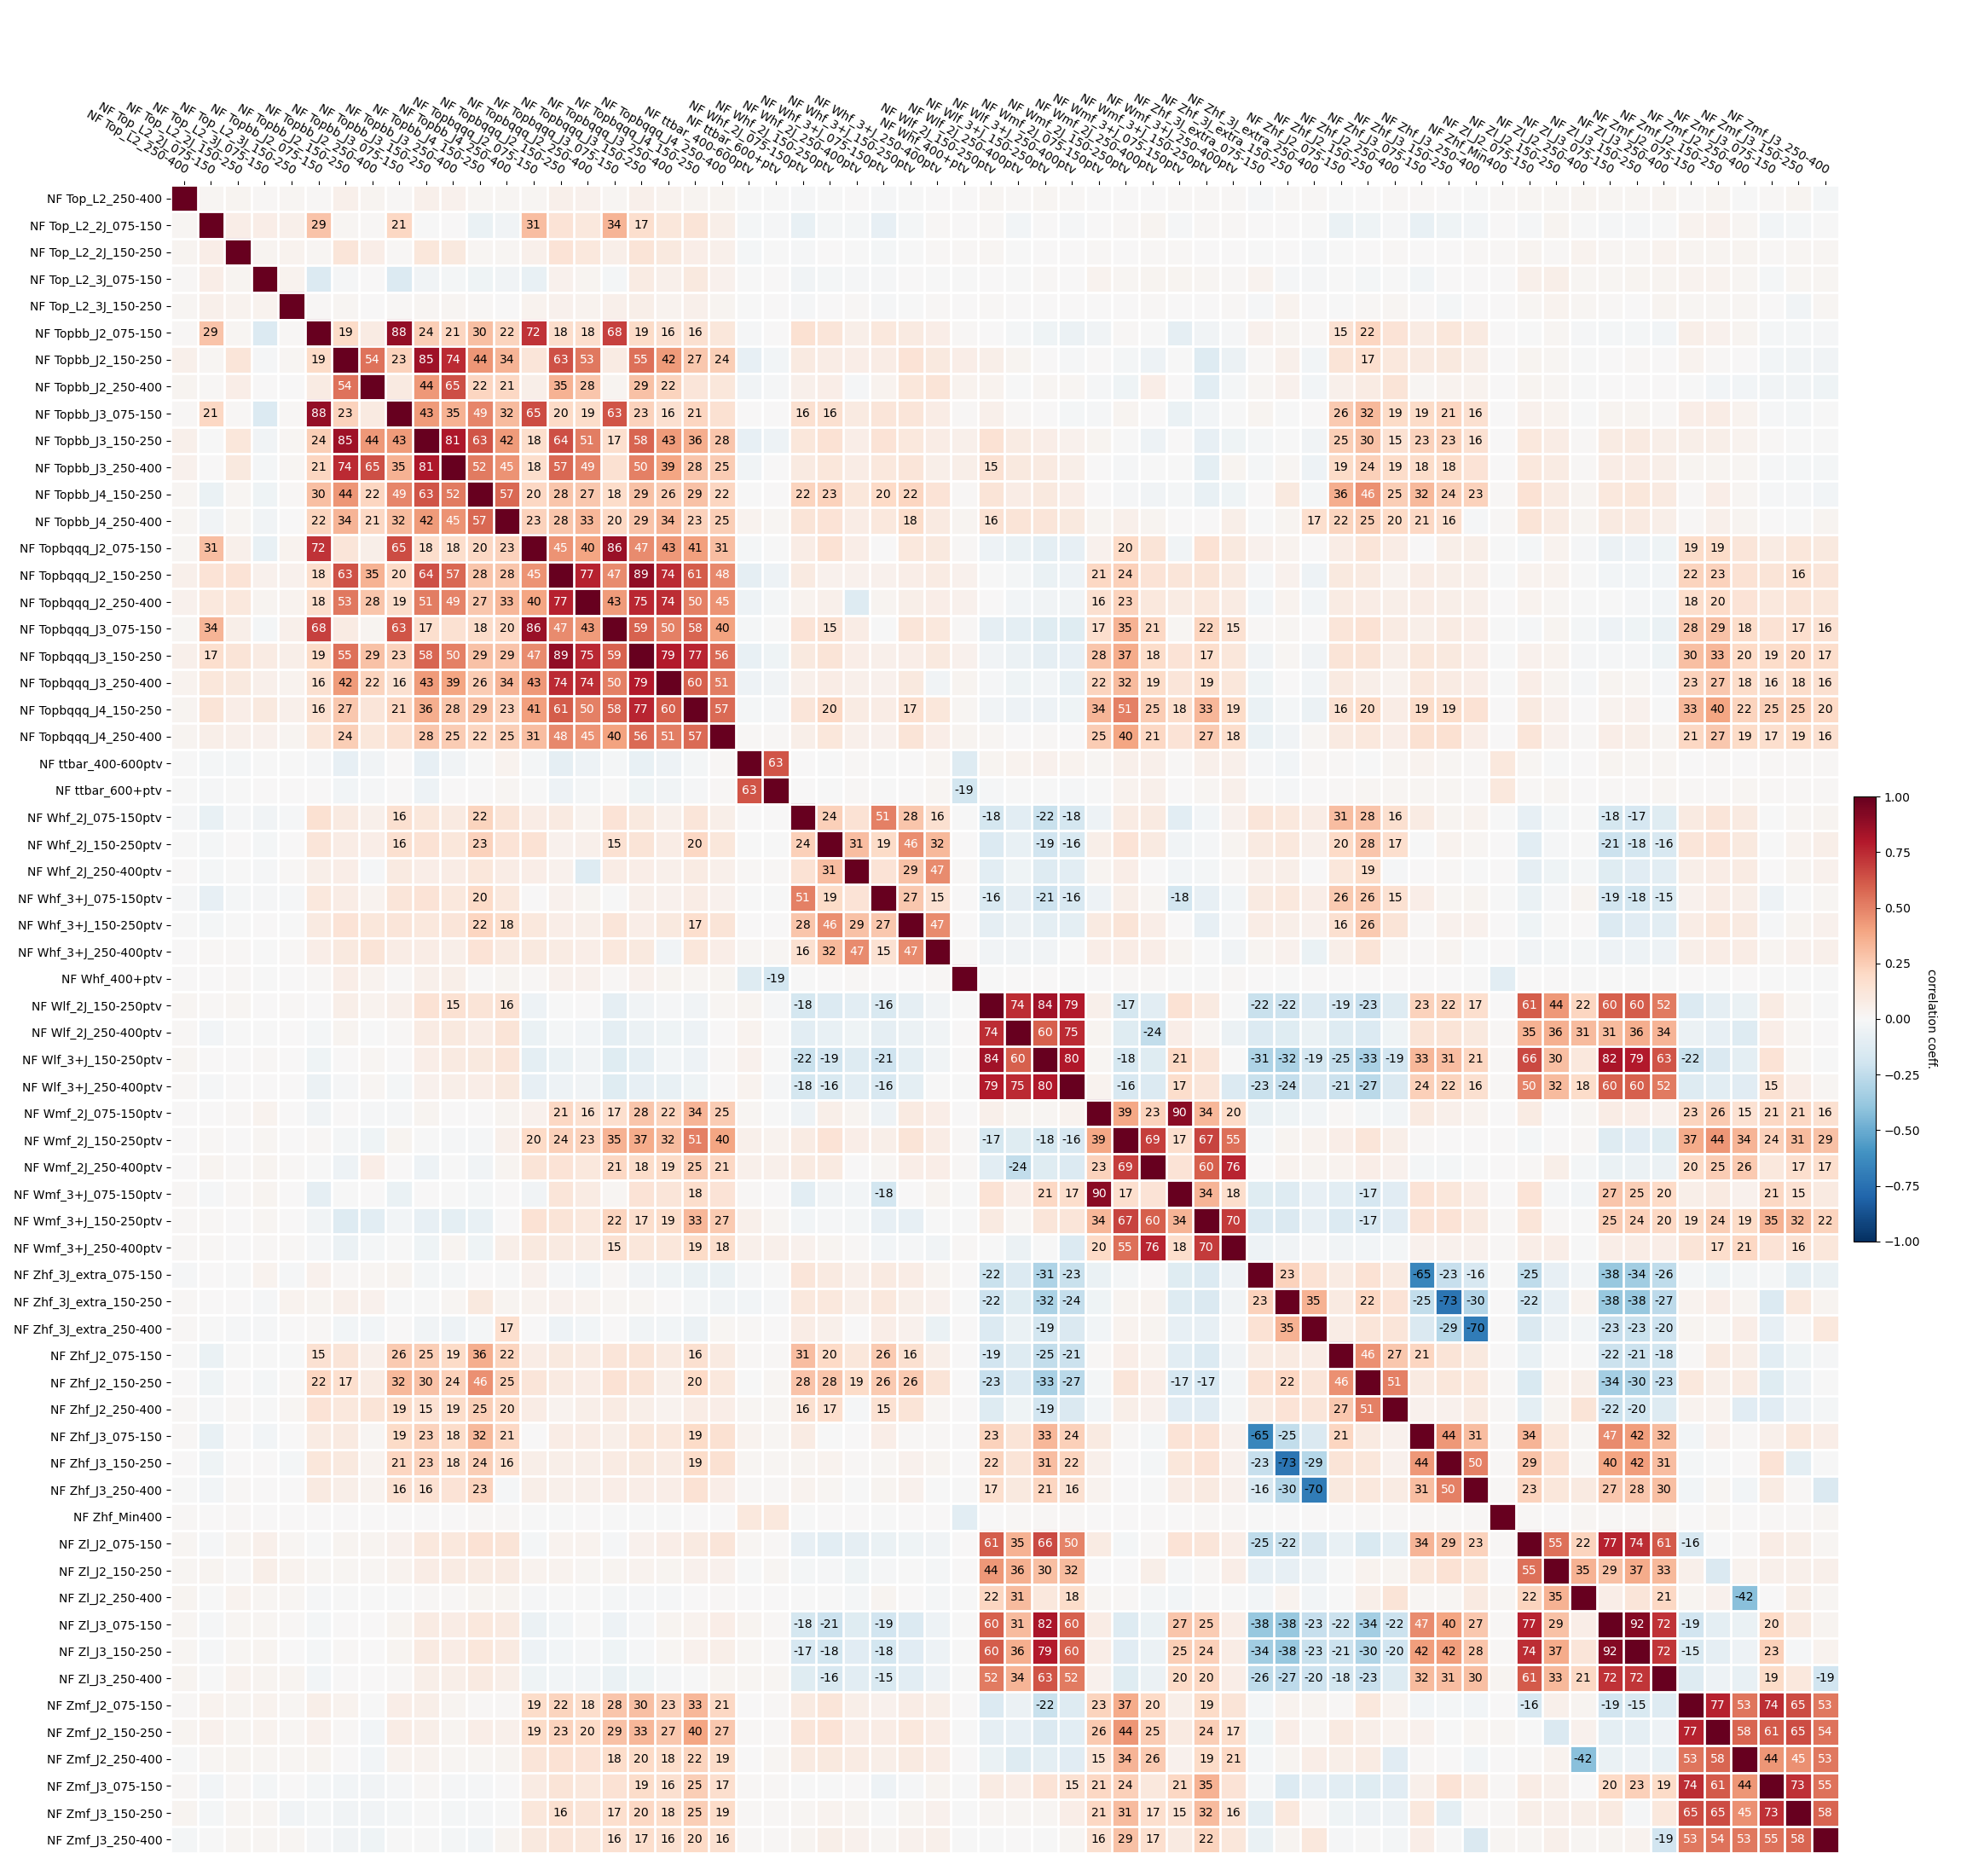
\includegraphics[width=1.1\textwidth]{Images/VH/Fit/fromSlides/SMVHbbcc_2022_MVA_mc16ade_v14.fit_012_fullRes_VHbb_fit_012_012_mc16ade_Systs_mva_VHbbcc_AsimovFit_conditional_mu1_Cov_BTag}
    \caption{The correlations between the floating normalisations of the major background in the combined \vhbc\ analysis.}
    \label{fig:FNcorr}
\end{figure} 

\section{Conclusion}
This chapter introduces the \vhbc\ combined ATLAS analysis using the 140 fb$^{-1}$ of data collected during Run 2 (2015-2018), in its state after its third unblinding approval meeting. Events are separated based on their \ptv\ and the two highest tags of their jet or sub-jets into a resolved or boosted regime \vhb\ or \vhc. Tagging is performed with the machine learning-based \gls{dl1r}, and the ranking establishes a hierarchy of $b$-tagged $>$ tight $c$-tagged $>$ loose $c$-tagged $>$ untagged. This is followed by a split into leptonic channel based on the number of charged lepton ($e$, $\mu$) in the final state, to separate the $Z(\rightarrow \nu\nu)H$, $W(\rightarrow \ell\nu)H$, and $Z(\rightarrow \ell^+\ell^-)H$, with the $H \rightarrow b\bar{b}$ or $H \rightarrow c\bar{c}$. To boost the sensitivity, a final categorisation further splits the analysis phase space into regions of defined \ptv\ and jet multiplicity. The major backgrounds of the analysis are the $V+$jets and the top processes, such as the \ttb\ pair production and the single-top $Wt$ production. These are respectively constrained from data in dedicated control regions defined by a cut on the angular separation of the Higgs-candidate jets and by an alternative event-tagging selection. To validate the adopted strategy, a cross-check analysis targeting the $VZ (\rightarrow b\bar{b}/c\bar{c})$ is performed. \\

The analysis promises to deliver exciting improvements in the sensitivity of the search for the $H\rightarrow c\bar{c}$ process, and the finest measurements to date of the differential cross-section of the \vhb. The analysis has already converged on the complex and wide-ranging categorisation strategy presented in this thesis. \gls{mva} discriminants are introduced throughout the different regimes to improve the sensitivity to the sought signals. The adoption of upgraded flavour tagging offered the opportunity to adopt a pseudo-continuous joint-tagging approach, paving the way for more coherent joint measurements of the $VH$ to heavy flavour quarks decay. New Monte-Carlo simulated samples of higher statistics contributed to reducing the importance of uncertainties plaguing the final fit performance. The final step, still under study at the time of writing by the analysis team, is to continue updating the modelling approach adopted to constrain the background within the limited knowledge of the detector and simulation uncertainties. Fine adjustments are required to understand how the complex fit introduced in this thesis constrains the different backgrounds, and whether this constraining is relying on physically motivated effects modelled by their respective nuisance parameters.\\

This analysis serves as the join combined legacy \vhb\ and \vhc\ analyses of ATLAS for the full Run 2, using the entire data statistics available of 140 fb$^{-1}$. Excitingly, progress in the analysis sensitivity to the \vhc\ signal strength has greatly accelerated, with reductions in the upper limit fast approaching the realm of direct measurement of the central value. At the current pace of improvement, the signal strength might be measurable in the next phase of the \gls{lhc}: the High-Luminosity-\gls{lhc} (HL-LHC). This will require continued improvement in the experimental tools and the analysis strategy. The former will primarily rely on improved flavour tagging abilities which, excitingly, is right around the corner for the $VH$ analysis: from the single tagger \gls{gn2} to the boosted $X \rightarrow b\bar{b} / c\bar{c}$ decay tagger \textit{GN2X}. The adoption of transformer-based neural networks is promising a significant increase in tagging performance. This will reverberate into an improved signal acceptance and a better separation from the backgrounds. The larger volume of data to be collected in Run 4 of the \gls{lhc} and future data-taking campaigns will significantly enrich the prospects of this severely statistically-limited analysis. This comes with an additional challenge, to operate at higher pile-ups, which will require additional upgrades to the experimental techniques, particularly in pile-up jets rejection. 